\documentclass[12pt,twoside, a4paper, twocolumn]{article}
\usepackage[utf8]{inputenc}
\usepackage[brazil]{babel}
\usepackage[margin = 0.5in]{geometry}
\usepackage{amsmath}
\usepackage{amsthm}
\usepackage{amssymb}
\usepackage{amsthm}
\usepackage{setspace}
\usepackage[americanvoltages,fulldiodes,siunitx]{circuitikz}
\usepackage{lipsum}
\usepackage{pgfplots}
\usepackage{ifthen}
\usepackage{adjustbox}
\usepackage[section]{placeins}
\usepackage{hyperref}
\usepackage{graphicx}
\usepackage{amsmath}
\usepackage{amsthm}
\usepackage{amssymb}
\usepackage{amsthm}
\usepackage{setspace}
\usepackage[americanvoltages,fulldiodes,siunitx]{circuitikz}
\usepackage{lipsum}
\usepackage{pgfplots}
\usepackage{ifthen}
\usepackage{adjustbox}
\usepackage[section]{placeins}
\usepackage{hyperref}
\usepackage{graphicx}
\usepackage{adjustbox}
 
\pgfplotsset{compat=newest}
 
\graphicspath{ {./images/} }
 
%  #1 color - optional #2 x_0 #3 y_0 #4 x_f #5 y_f #6 name - optional  #7 true if adding lines to axis
 
\newcommand{\drawvector} [9] [color=cyan] {
   \draw[line width=1.5pt,#1,-stealth](axis cs: #2, #3)--(axis cs: #4, #5) node[anchor=south west]{$#6$};
 
  
 
\ifthenelse{\equal{#7}{true}}{
   \draw[line width=1pt,#1, dashed](axis cs: #4, #5)--(axis cs: #4, 0) node[anchor= north west]{$#8$};
   \draw[line width=1pt,#1, dashed](axis cs: #4, #5)--(axis cs: 0, #5) node[anchor=south east]{$#9$};
   }
   {}
}
 
\newcommand\deriv[2]{\frac{\mathrm d #1}{\mathrm d #2}}
 
 
\title{Segundo Relatório de Lab de Circuitos II}
\author{Henrique da Silva \\ hpsilva@proton.me}
\date{\today}
\pgfplotsset{width = 10cm, compat = 1.9}
 
 
\begin{document}
\maketitle
\pagenumbering{gobble}
\newpage
%pagenumbering{roman}
\tableofcontents
\newpage



\section{Introdução}


\subparagraph*{Neste relatório, vamos discutir a funcao transferencia na resposta em regime permanente senoidal de um circuito.}

\subparagraph*{Todos arquivos utilizados para criar este relatorio, e o relatorio em si estão em:  \url{https://github.com/Shapis/ufpe_ee/tree/main/5th semester/Electromagnetic Measurements/Relatorios}}




\section{Análise preliminar}

\paragraph*{Utilizarei o WxMaxima e LTSpice para fazer a analise teorica do circuito antes de monta-lo fisicamente.}

\paragraph*{Apos terminar as analises compararei os resultados obtidos entre os dois para ver se os resultados sao coerentes.}

\subsection{O Circuito}
\begin{adjustbox}{scale=0.30}
    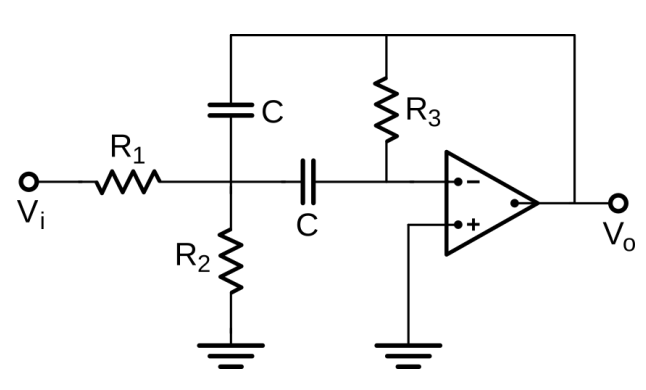
\includegraphics{AnaliseNodal.png}
\end{adjustbox}
\newpage
\subsection{WxMaxima}

\subparagraph*{Primeiro fiz manualmente a analise nodal do circuito que vamos construir, e passei ele para o dominio da frequencia.}
\subparagraph*{}

\begin{adjustbox}{scale=0.26}
    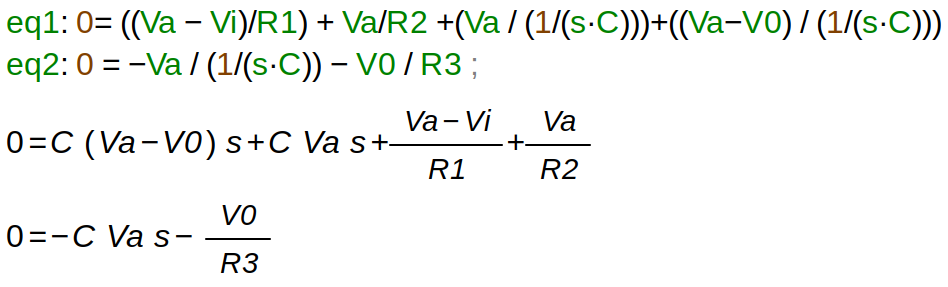
\includegraphics{eqs.png}
\end{adjustbox}

\subparagraph*{Apos isso resolvi para $Va$ e $V_0$}

\subparagraph*{}

\begin{adjustbox}{scale=0.33}
    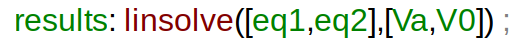
\includegraphics{linsolve.png}
\end{adjustbox}

\begin{adjustbox}{scale=0.33}
    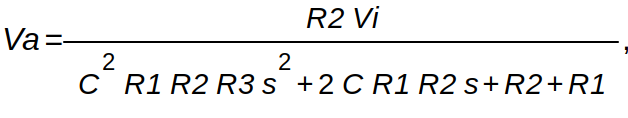
\includegraphics{va.png}
\end{adjustbox}

\begin{adjustbox}{scale=0.33}
    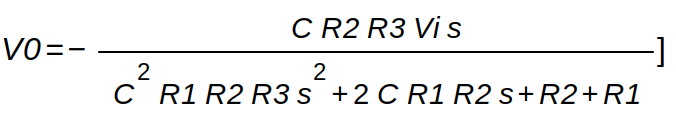
\includegraphics{v0.png}
\end{adjustbox}

\subparagraph*{Daqui criamos nossa funcao transferencia $H$.}

\subparagraph*{}

\begin{adjustbox}{scale=0.33}
    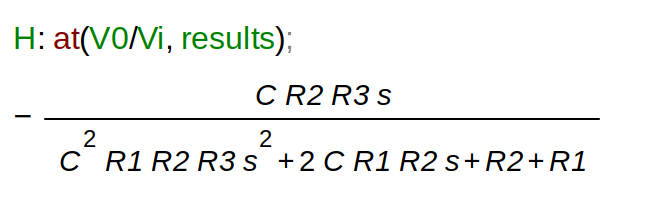
\includegraphics{H.png}
\end{adjustbox}

\subparagraph*{Apos isso fiz a substituicao $S = iw$ para poder calcular a magnitude e seu angulo de fase.}

\subparagraph*{}

\begin{adjustbox}{scale=.17}
    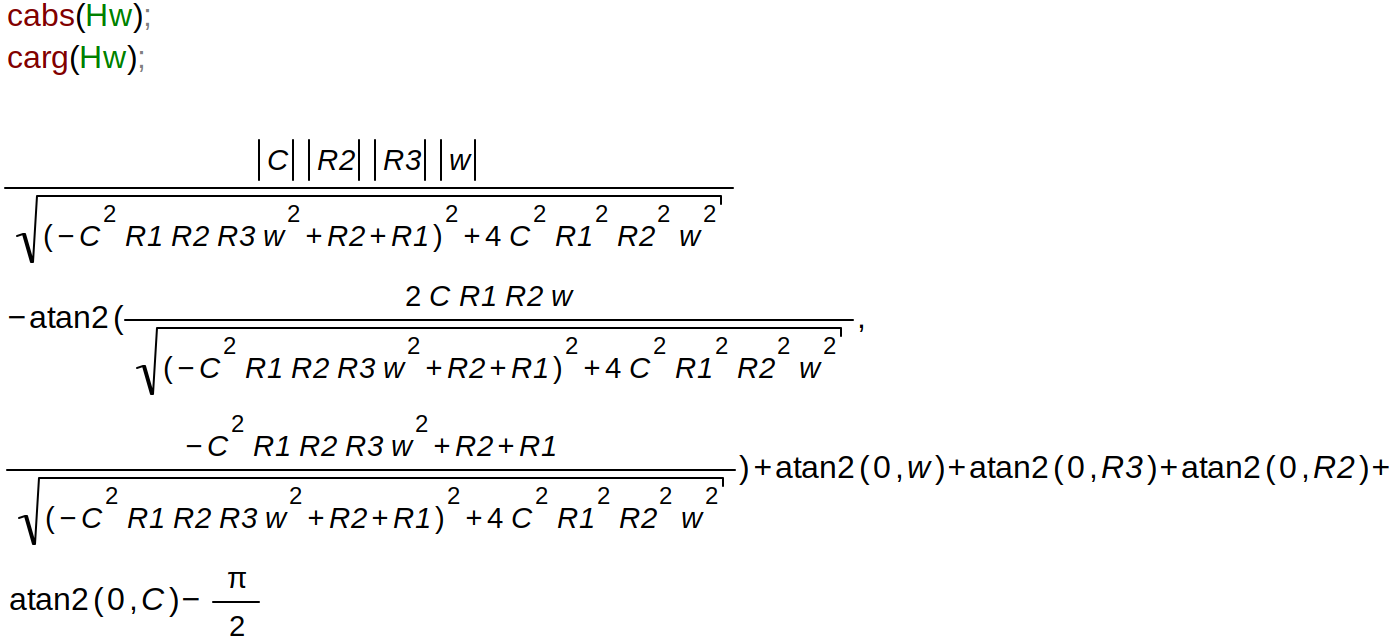
\includegraphics{sjw.png}
\end{adjustbox}

\subparagraph*{Agora com a funcao $Hw$ em maos podemos substituir os valores dos resistores e do capacitor pelos que utilizaremos.}

\begin{adjustbox}{scale=0.30}
    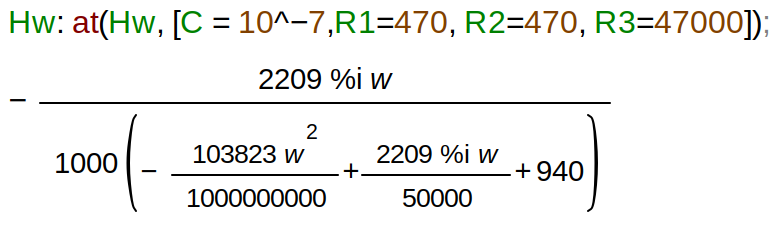
\includegraphics{substituicao.png}
\end{adjustbox}

\subparagraph*{Como nosso objetivo eh analisar a magnitude e o angulo de fase da funcao transferencia, podemos extrair disto a parte real e imaginaria da equacao acima.}

\subparagraph*{}

\begin{adjustbox}{scale=0.21}
    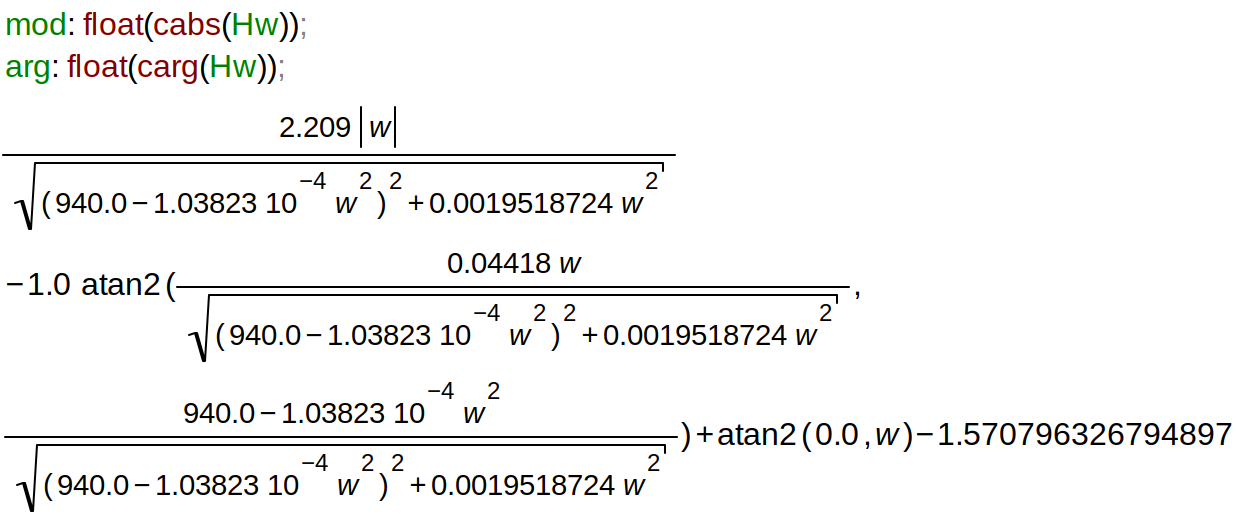
\includegraphics{modarg.png}
\end{adjustbox}

\subparagraph*{E Finalmente com estas funcoes em maos, substitui a frequencia com as frequencias pedidas.}

\subparagraph*{}

\begin{adjustbox}{scale=0.30}
    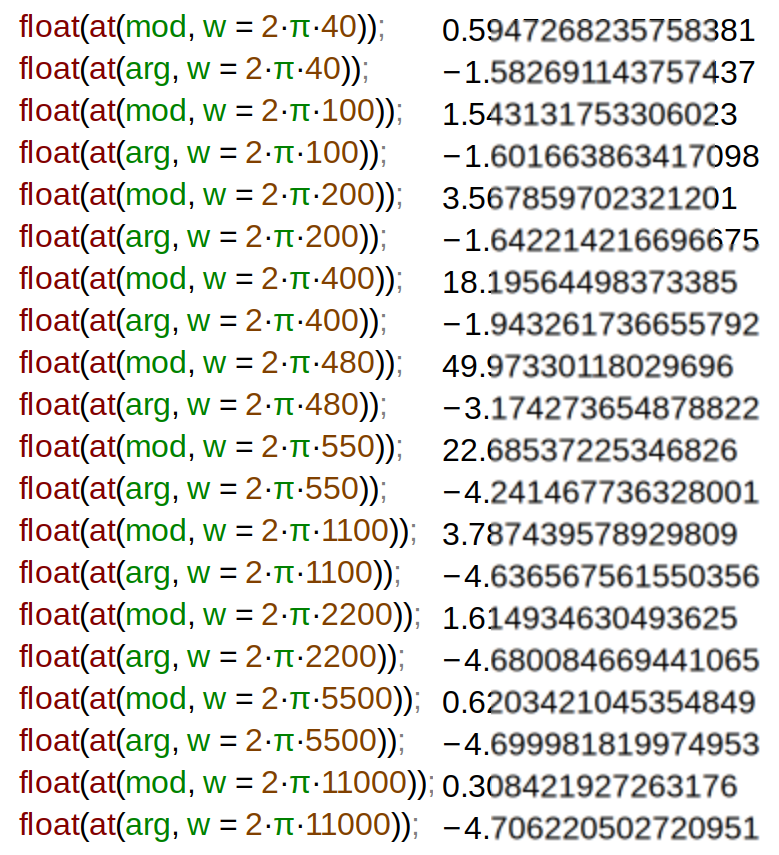
\includegraphics{resultados.png}
\end{adjustbox}

\subparagraph*{Com isto temos em maos as magnitudes e angulos de fase da funcao transferencia para um gama de frequencias.}

\newpage

\subsection{LTSpice}

\paragraph*{No LTSpice montaremos o circuito e mediremos novamente o angulo de fase e sua magnitude.}
\subparagraph*{}
\begin{adjustbox}{scale=0.09}
    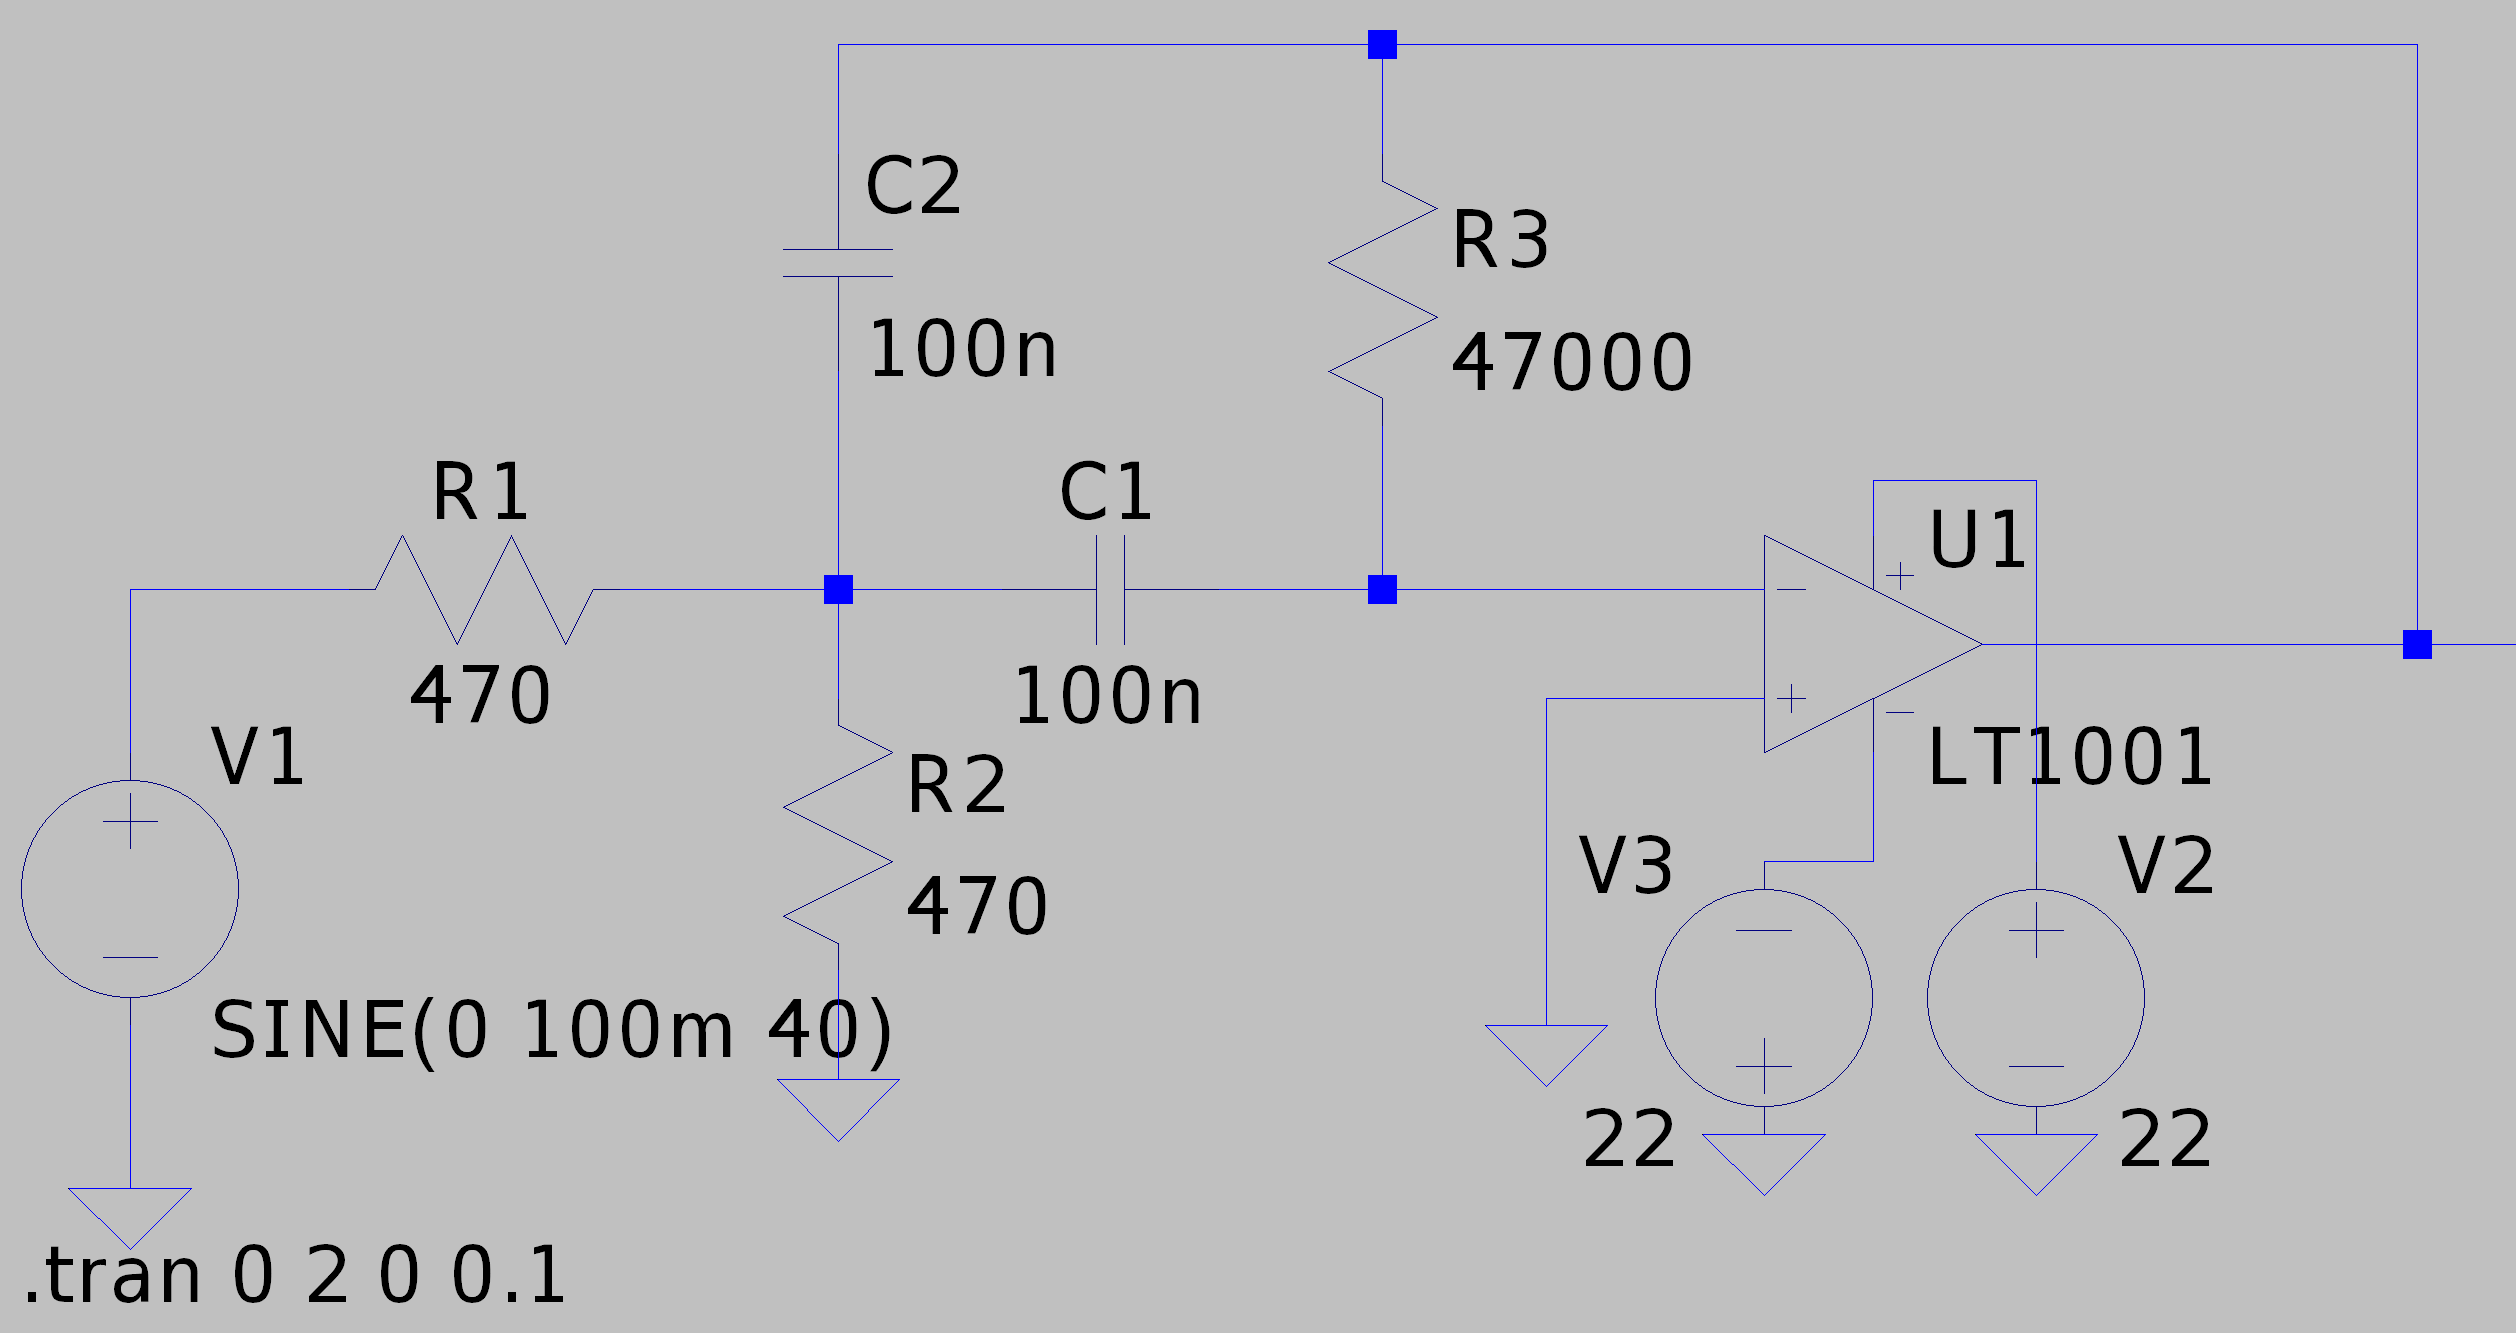
\includegraphics{ltspicecirc.png}
\end{adjustbox}

\subsubsection{Analise em $40Hz$}

\begin{adjustbox}{scale=0.09}
    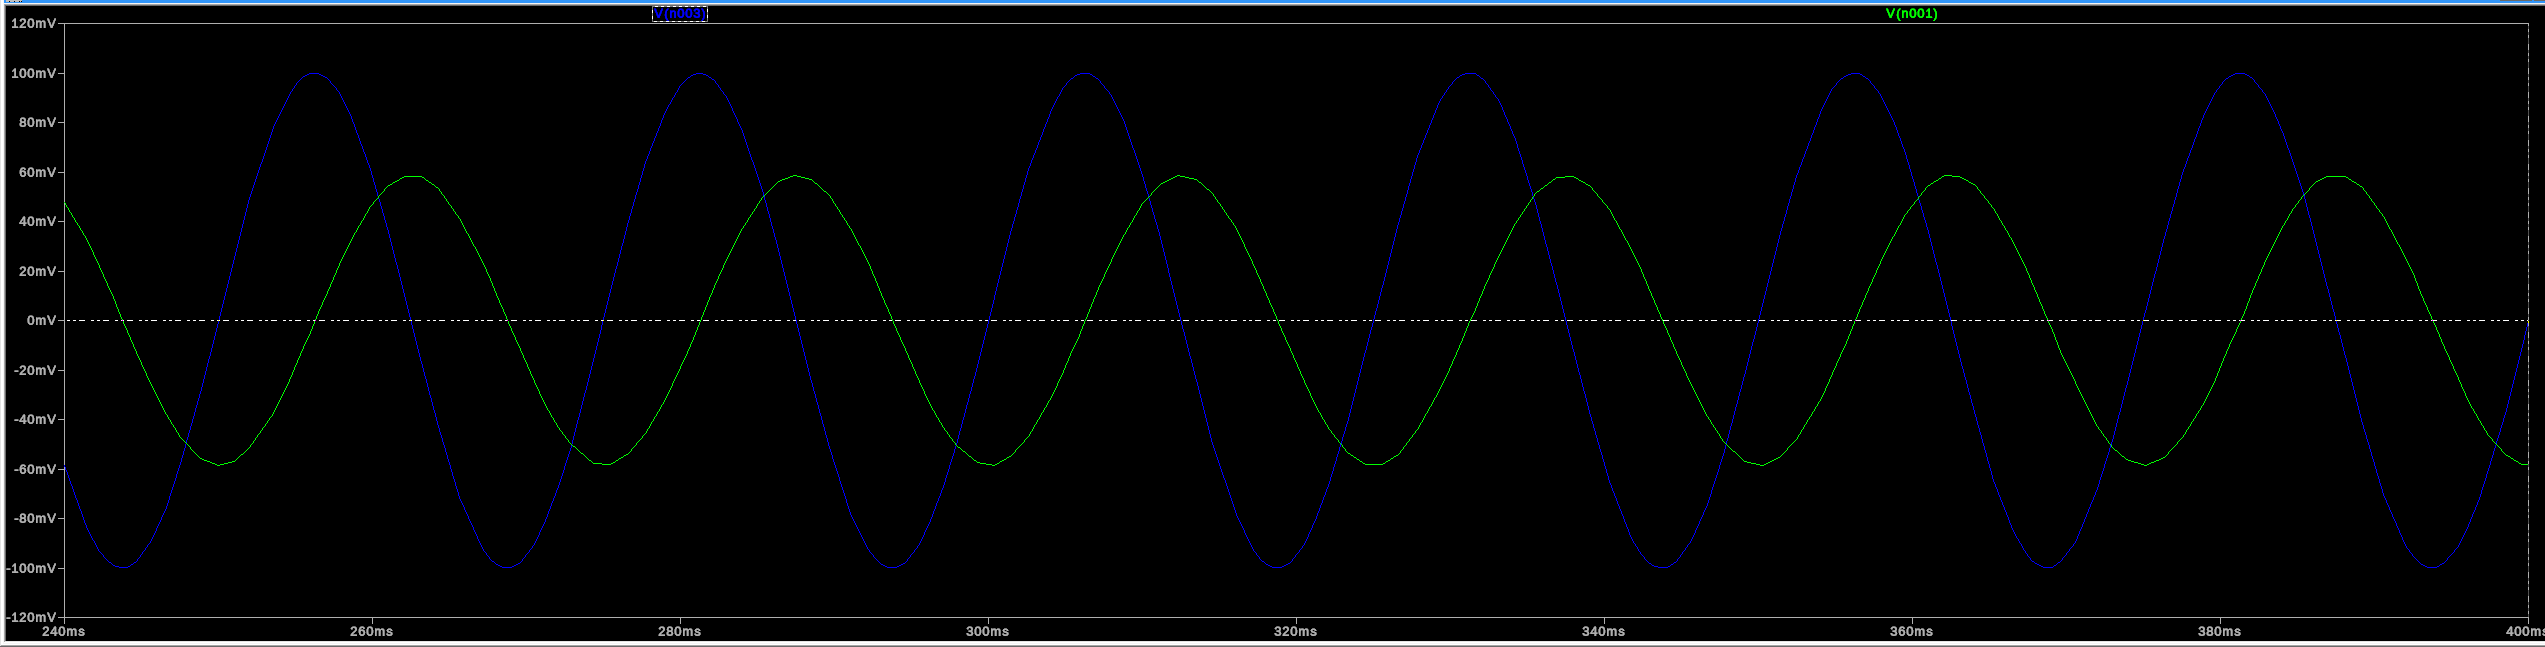
\includegraphics{ltfreq40.png}
\end{adjustbox}

\begin{equation*}
    \begin{aligned}
         & V_f =          & 117.10115mV \\
         & V_i =          & 199.76772mV \\
         & Magnitude(H) = & 0.586186547 \\
         & Fase =         & -1.68605608
    \end{aligned}
\end{equation*}

\subsubsection{Analise em $100Hz$}

\begin{adjustbox}{scale=0.09}
    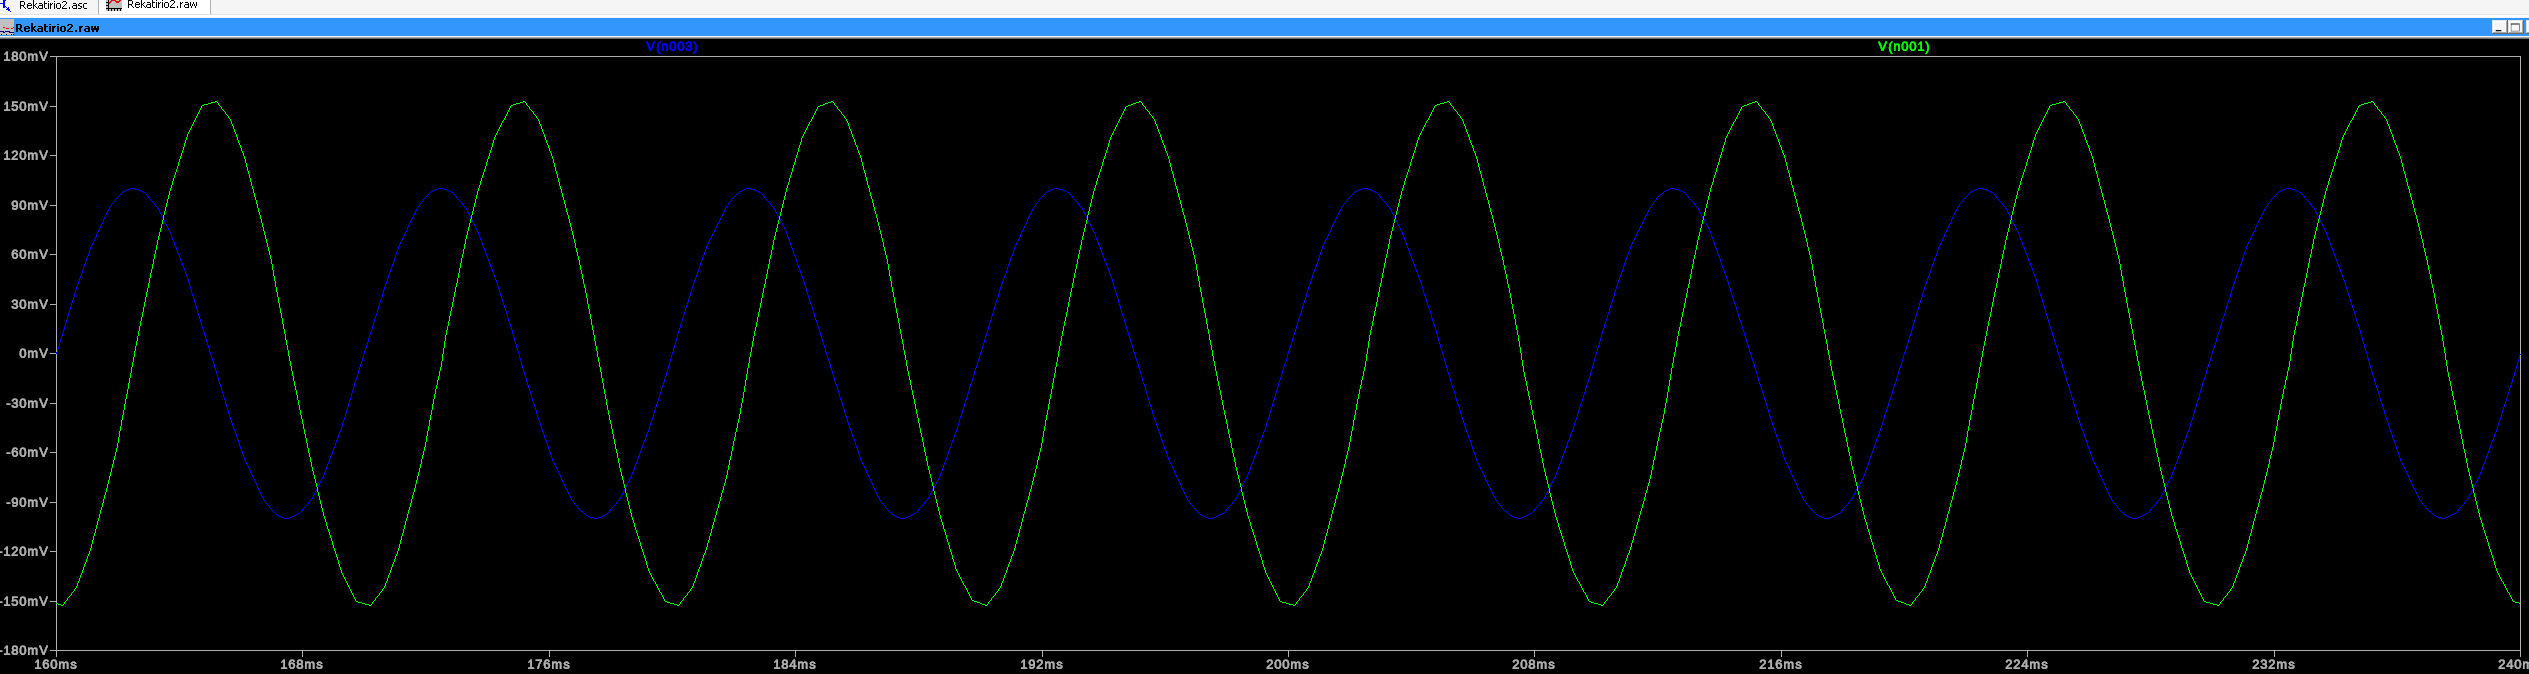
\includegraphics{ltfreq100.png}
\end{adjustbox}

\begin{equation*}
    \begin{aligned}
         & V_f =          & 303.64554mV \\
         & V_i =          & 199.34196mV \\
         & Magnitude(H) = & 1.52323946  \\
         & Fase =         & -1.60226153
    \end{aligned}
\end{equation*}


\subsubsection{Analise em $200Hz$}

\begin{adjustbox}{scale=0.09}
    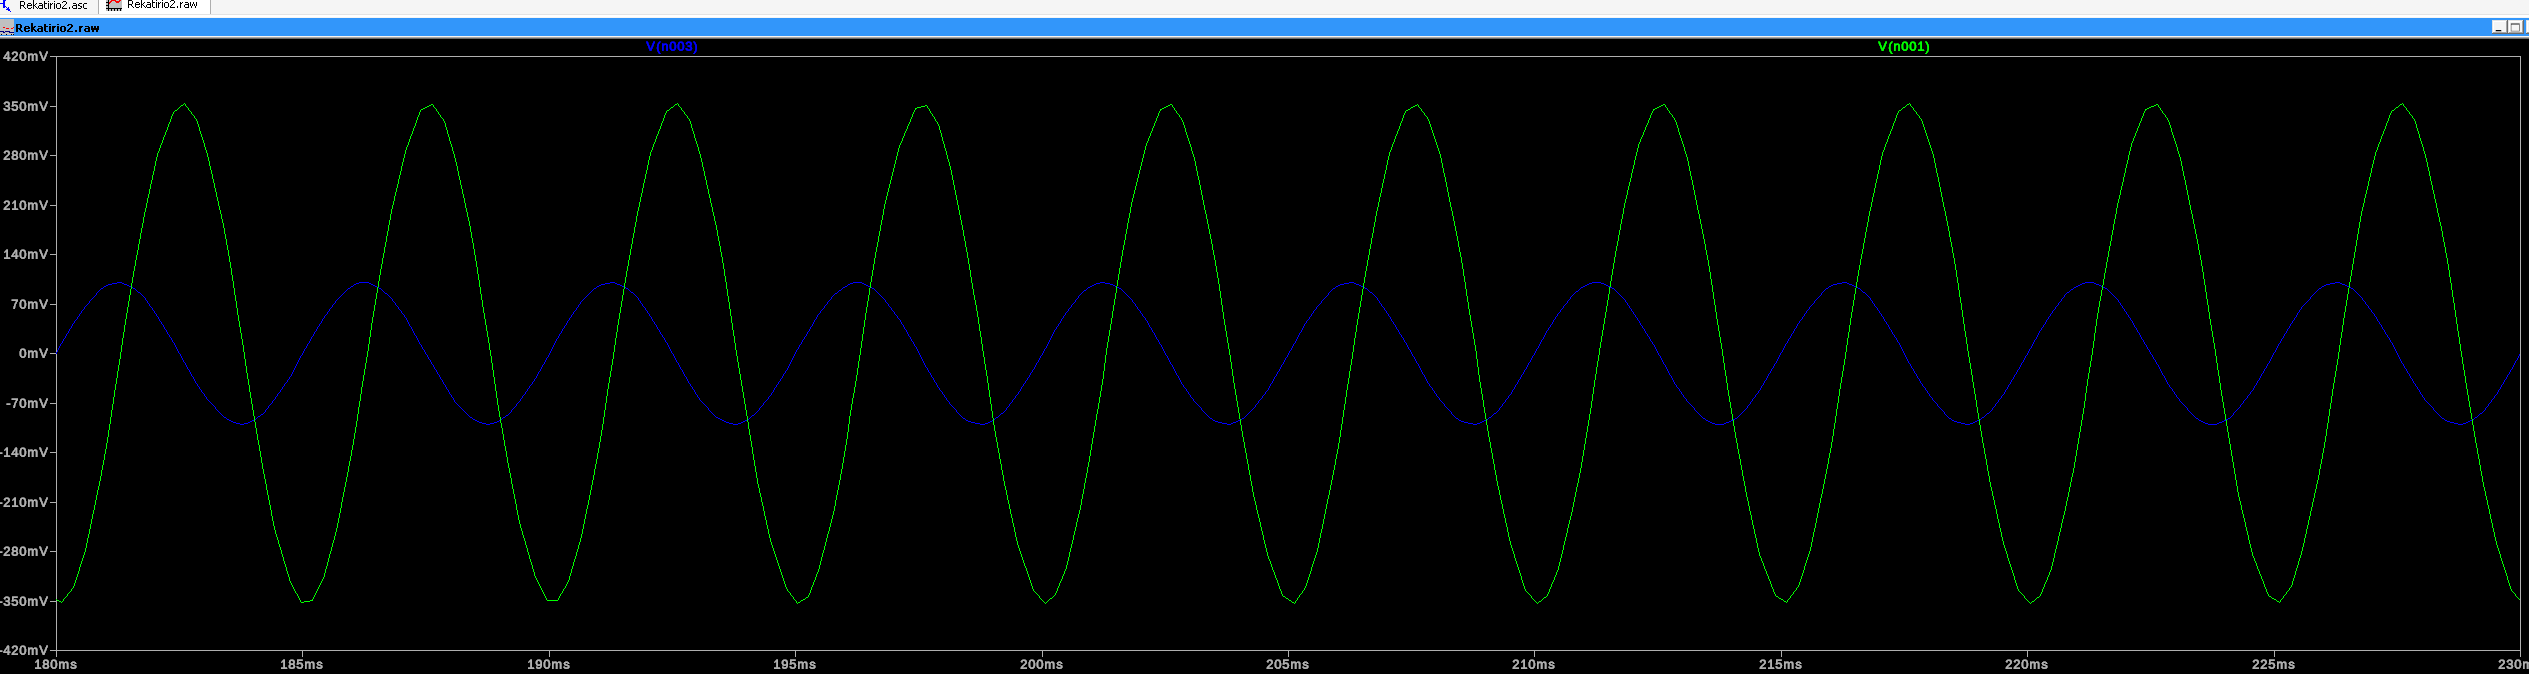
\includegraphics{ltfreq200.png}
\end{adjustbox}

\begin{equation*}
    \begin{aligned}
         & V_f =          & 704.6312mV  \\
         & V_i =          & 199.46039mV \\
         & Magnitude(H) = & 3.53268737  \\
         & Fase =         & -1.67119113
    \end{aligned}
\end{equation*}

\subsubsection{Analise em $400Hz$}

\begin{adjustbox}{scale=0.09}
    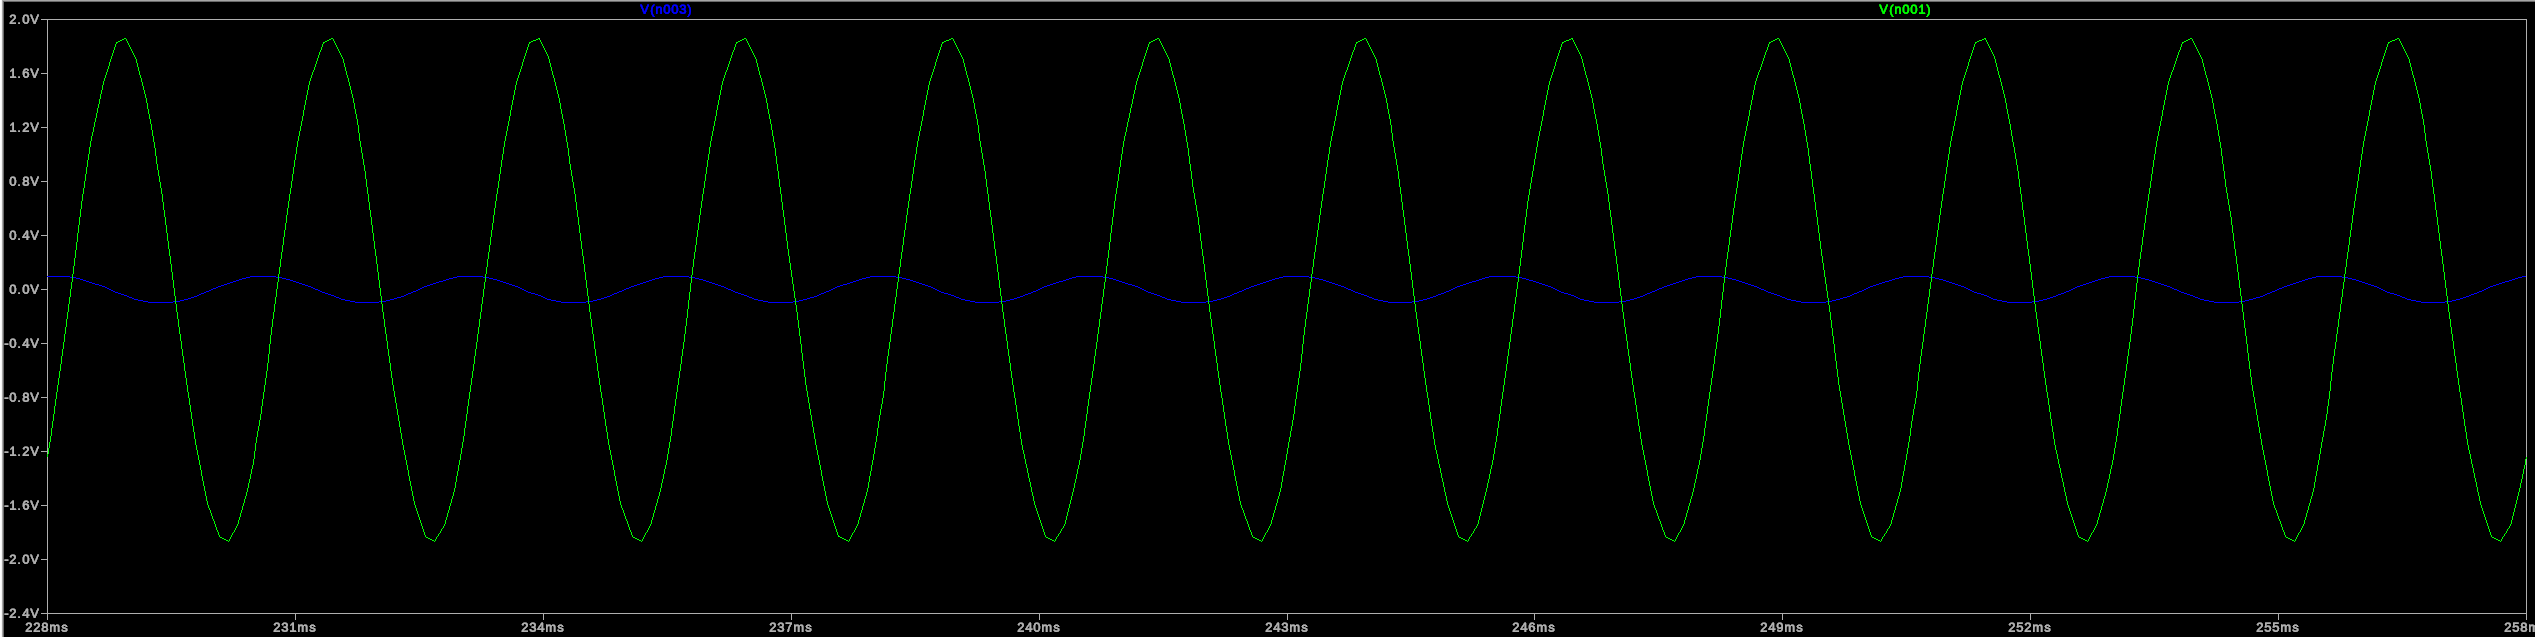
\includegraphics{ltfreq400.png}
\end{adjustbox}

\begin{equation*}
    \begin{aligned}
         & V_f =          & 3.7148299V  \\
         & V_i =          & 199.72118mV \\
         & Magnitude(H) = & 18.6104333  \\
         & Fase =         & -2.06820459
    \end{aligned}
\end{equation*}

\subsubsection{Analise em $480Hz$}

\begin{adjustbox}{scale=0.09}
    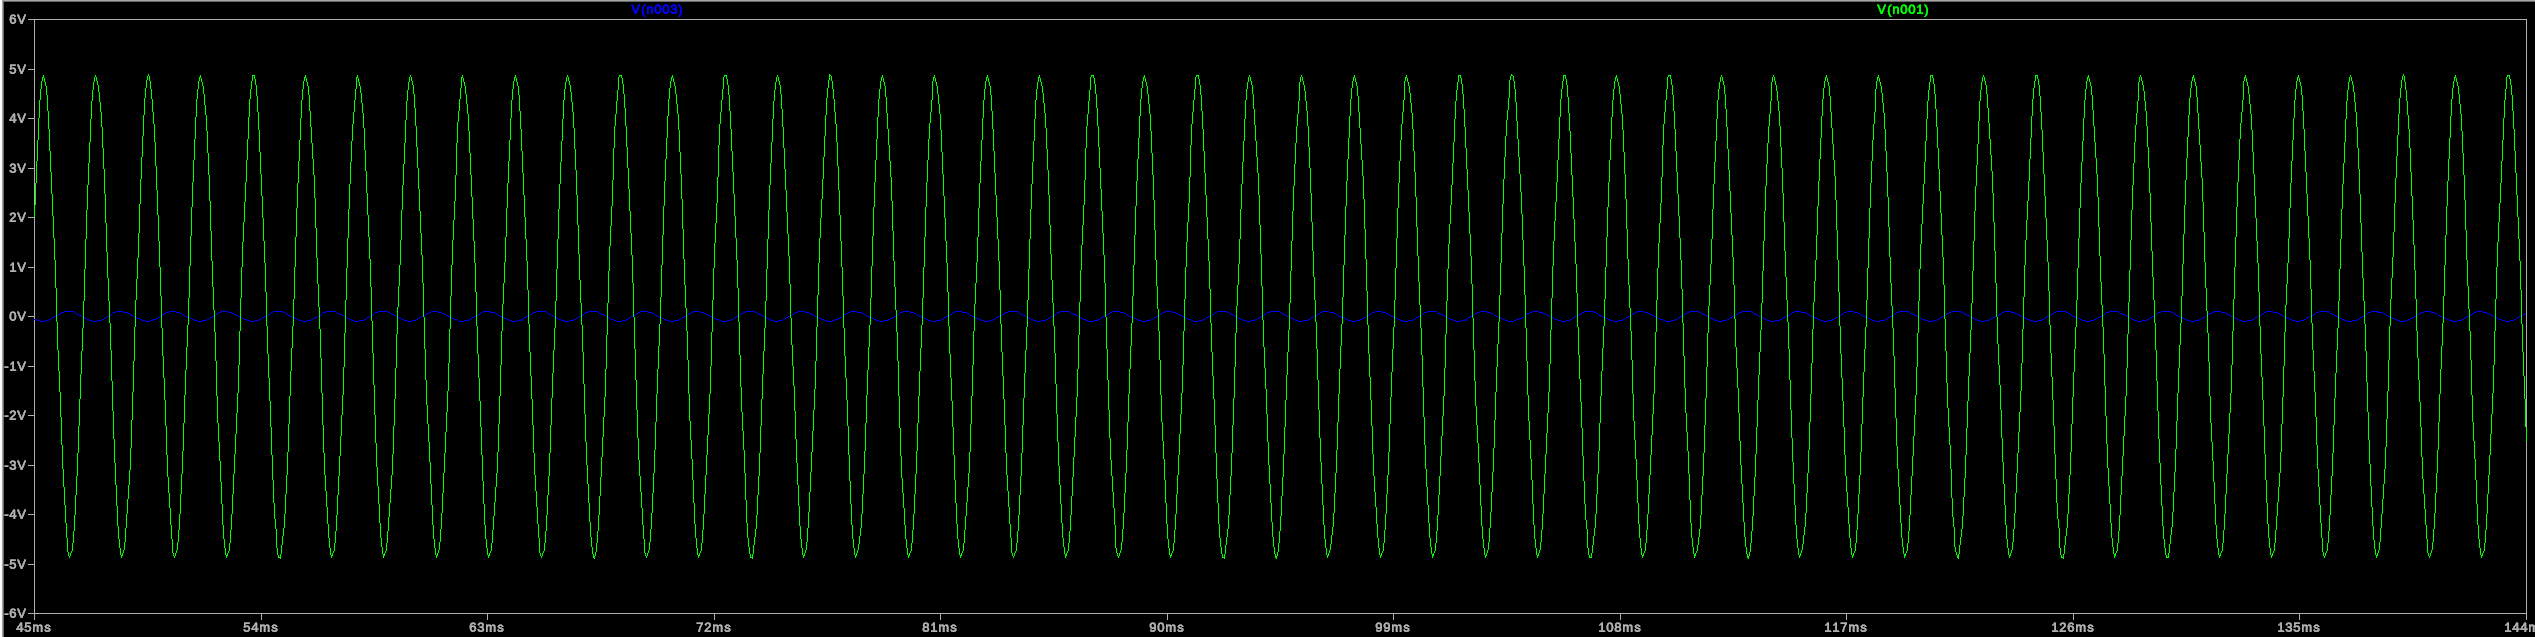
\includegraphics{ltfreq480.png}
\end{adjustbox}

\begin{equation*}
    \begin{aligned}
         & V_f =          & 9.7253442V  \\
         & V_i =          & 199.42436mV \\
         & Magnitude(H) = & 48.7670824  \\
         & Fase =         & -3.13491022
    \end{aligned}
\end{equation*}

\subsubsection{Analise em $550Hz$}

\begin{adjustbox}{scale=0.09}
    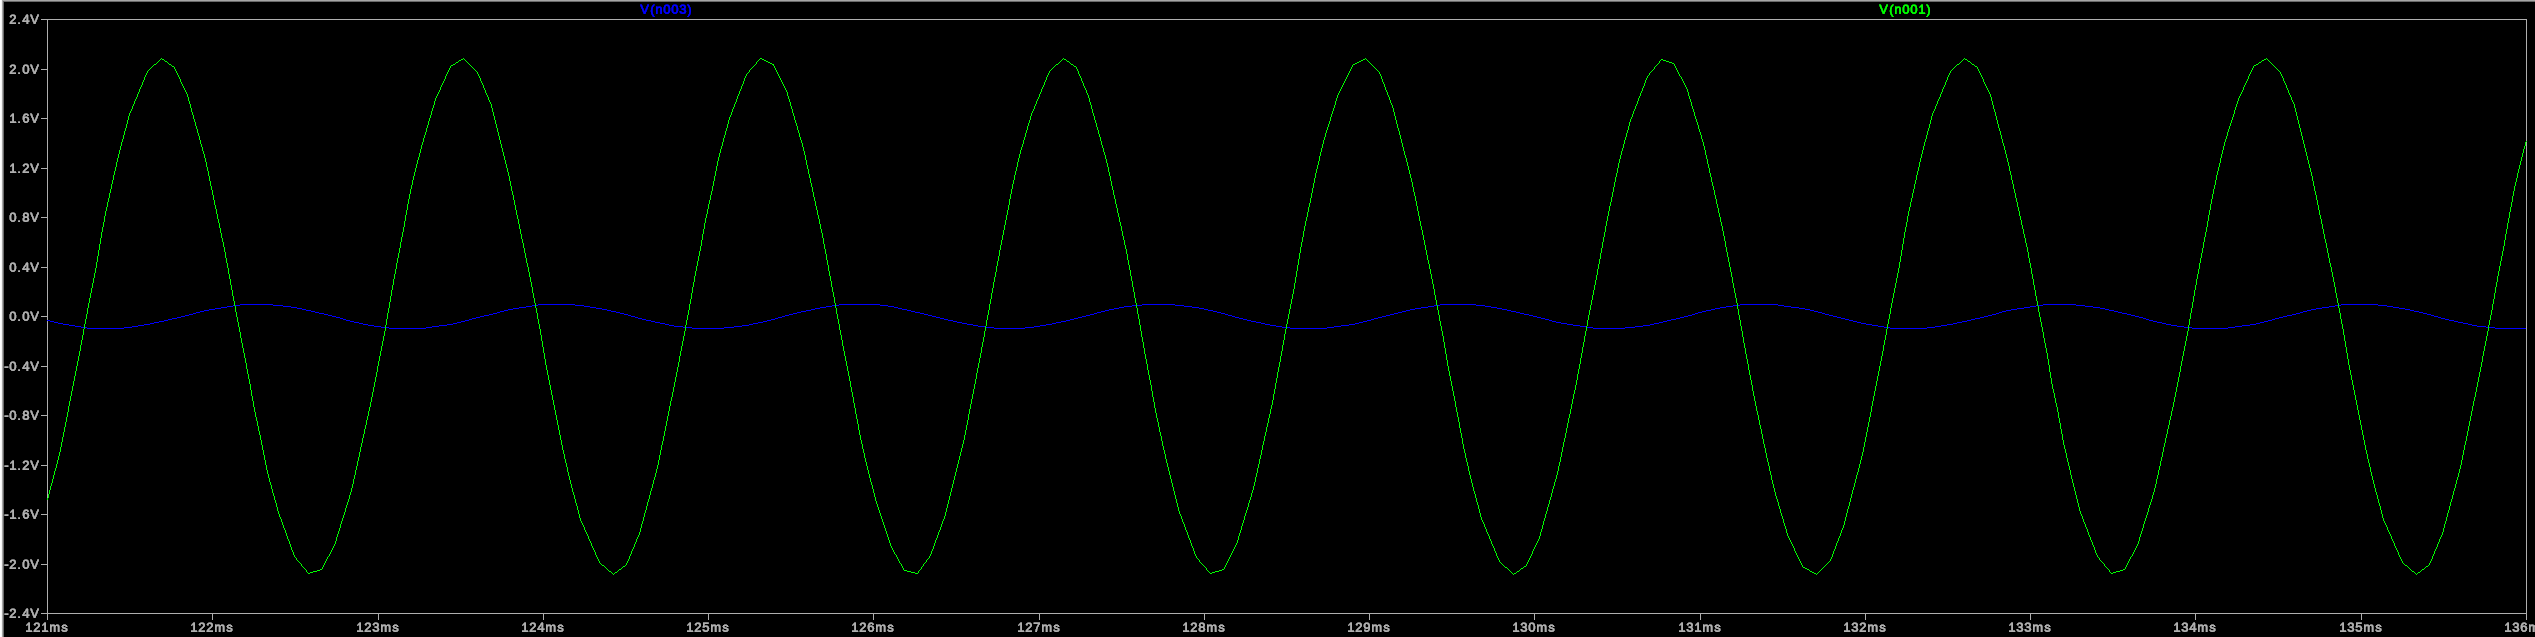
\includegraphics{ltfreq550.png}
\end{adjustbox}

\begin{equation*}
    \begin{aligned}
         & V_f =          & 4.1496957V  \\
         & V_i =          & 199.35122mV \\
         & Magnitude(H) = & 20.8160035  \\
         & Fase =         & -2.01155708
    \end{aligned}
\end{equation*}

\subsubsection{Analise em $1100Hz$}

\begin{adjustbox}{scale=0.09}
    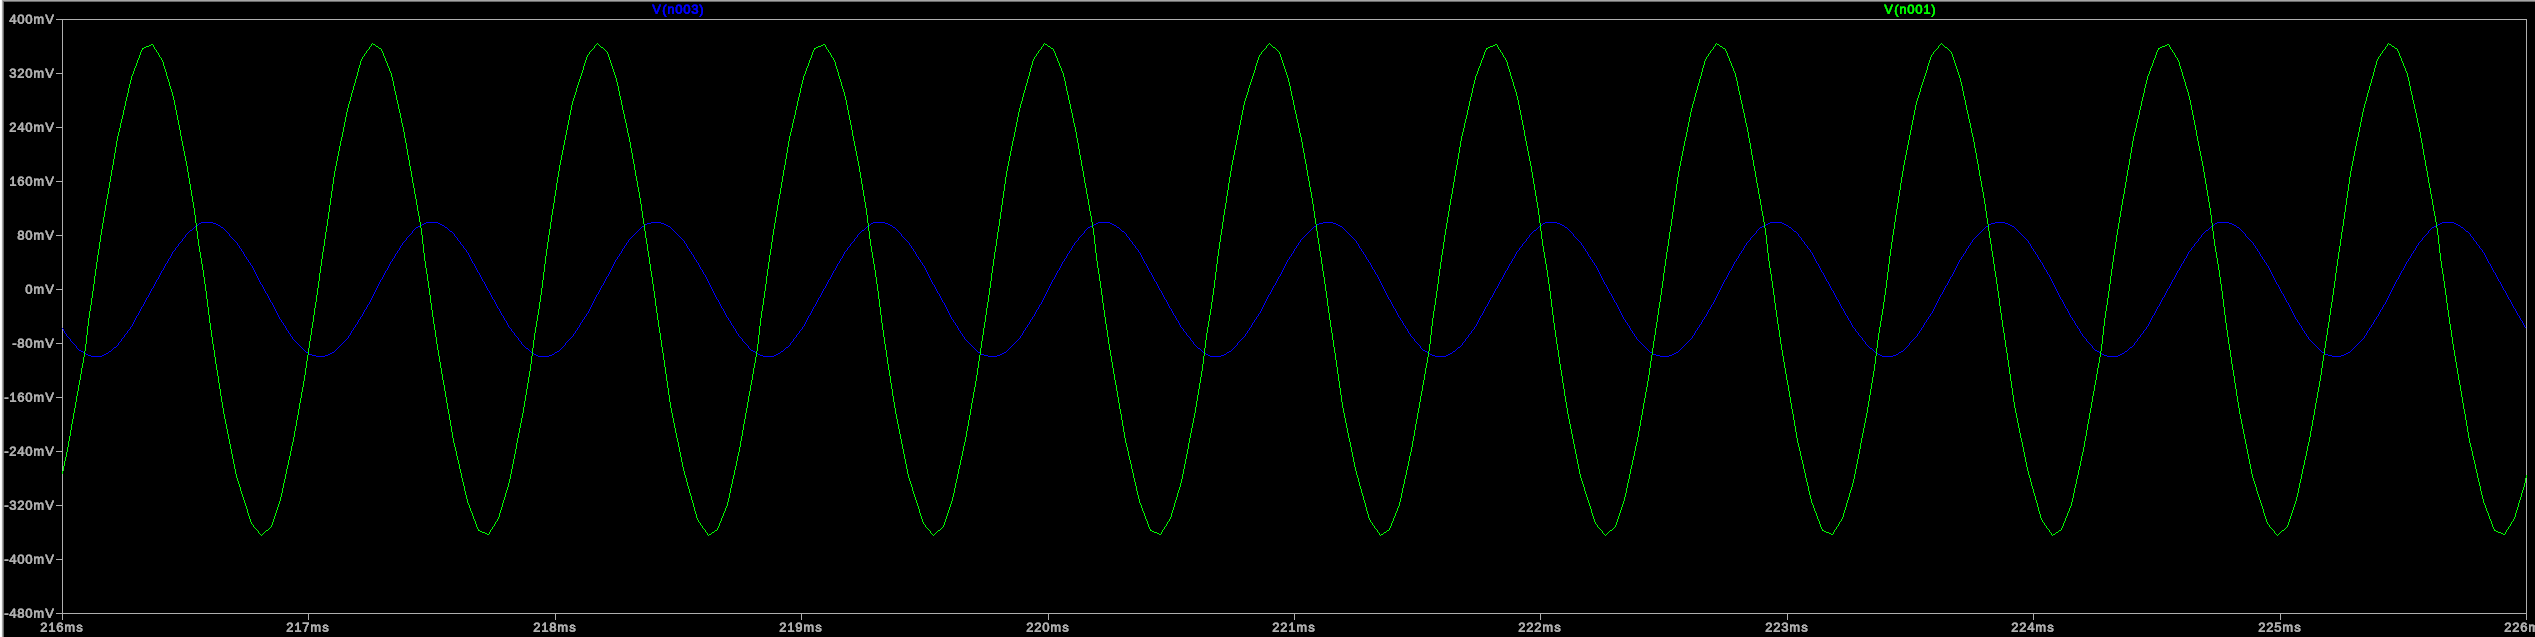
\includegraphics{ltfreq1100.png}
\end{adjustbox}

\begin{equation*}
    \begin{aligned}
         & V_f =          & 724.81506mV \\
         & V_i =          & 199.55853mV \\
         & Magnitude(H) = & 3.6320926   \\
         & Fase =         & -1.65494612
    \end{aligned}
\end{equation*}

\subsubsection{Analise em $2200Hz$}

\begin{adjustbox}{scale=0.09}
    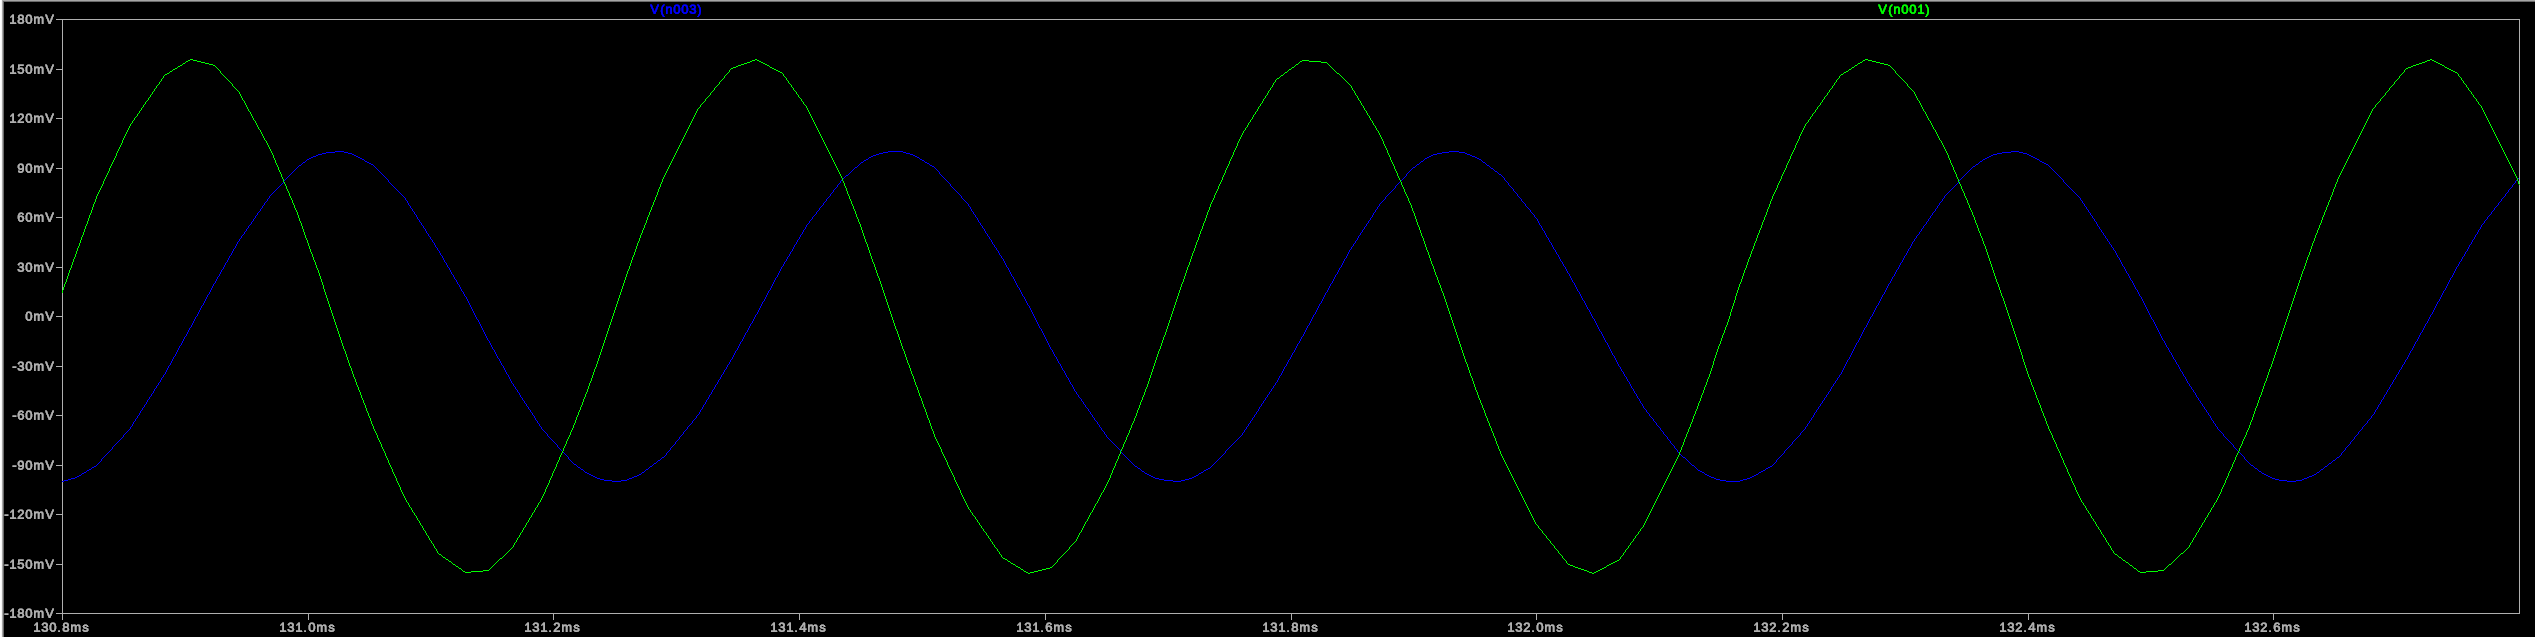
\includegraphics{ltfreq2200.png}
\end{adjustbox}

\begin{equation*}
    \begin{aligned}
         & V_f =          & 310.31854mV \\
         & V_i =          & 199.32175mV \\
         & Magnitude(H) = & 1.55687244  \\
         & Fase =         & -4.68032157
    \end{aligned}
\end{equation*}

\subsubsection{Analise em $5500Hz$}

\begin{adjustbox}{scale=0.09}
    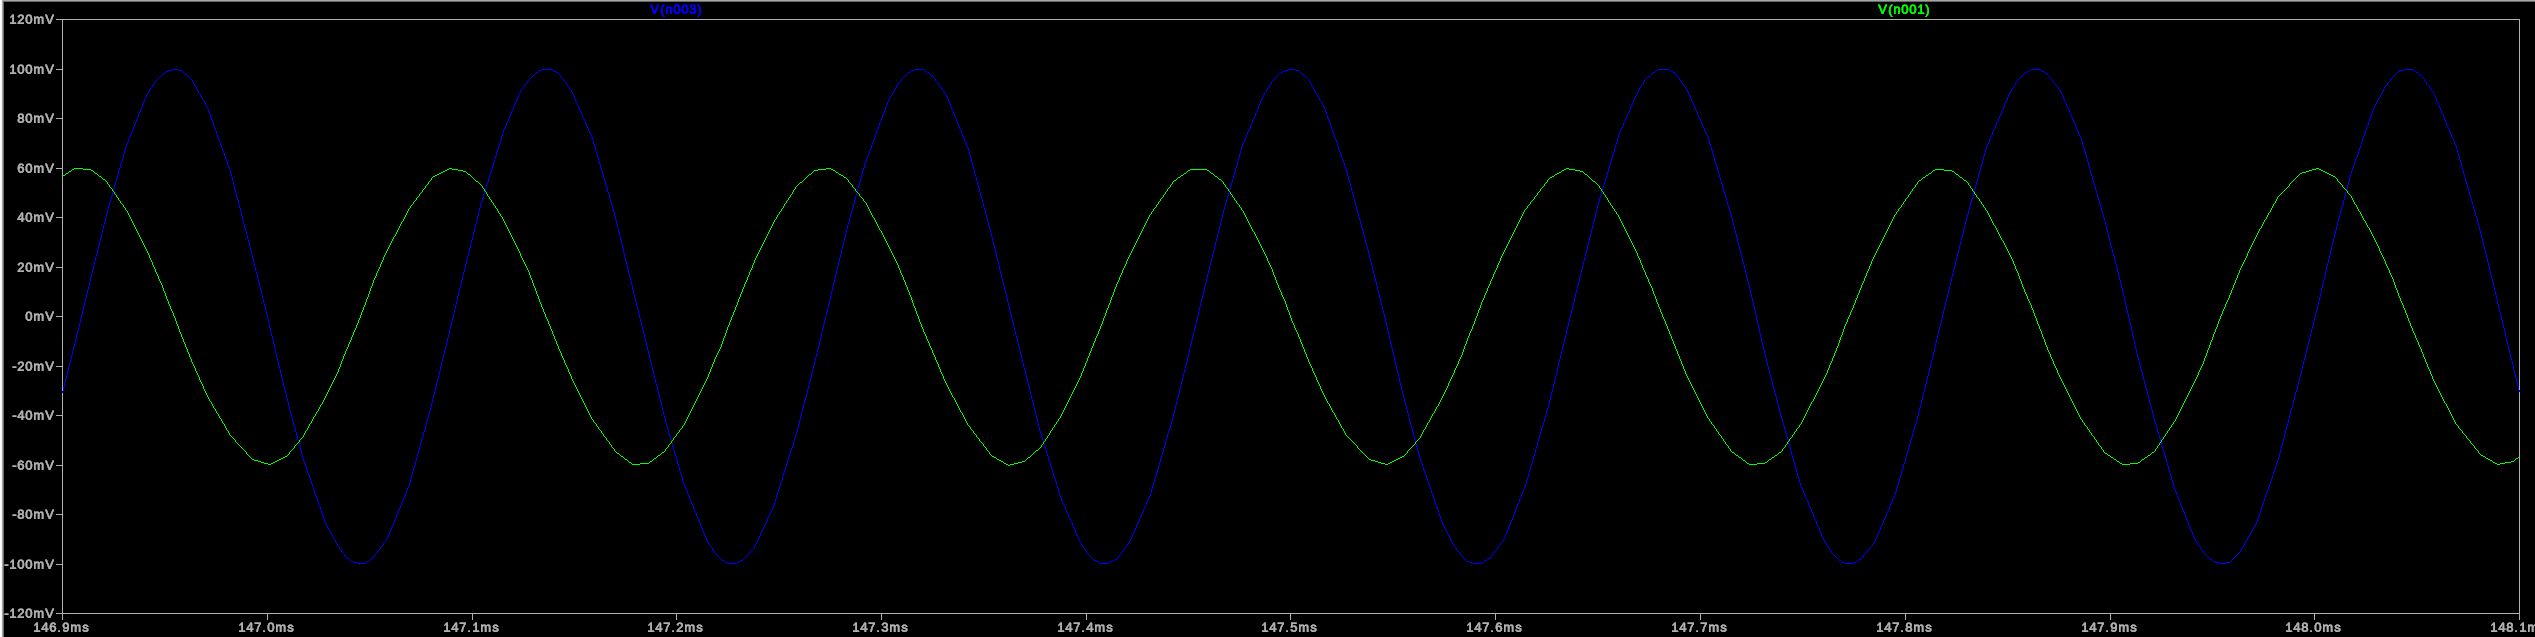
\includegraphics{ltfreq5500.png}
\end{adjustbox}

\begin{equation*}
    \begin{aligned}
         & V_f =          & 118.93005mV \\
         & V_i =          & 199.79451mV \\
         & Magnitude(H) = & 0.595261852 \\
         & Fase =         & 1.60939706
    \end{aligned}
\end{equation*}

\subsubsection{Analise em $11000Hz$}

\begin{adjustbox}{scale=0.09}
    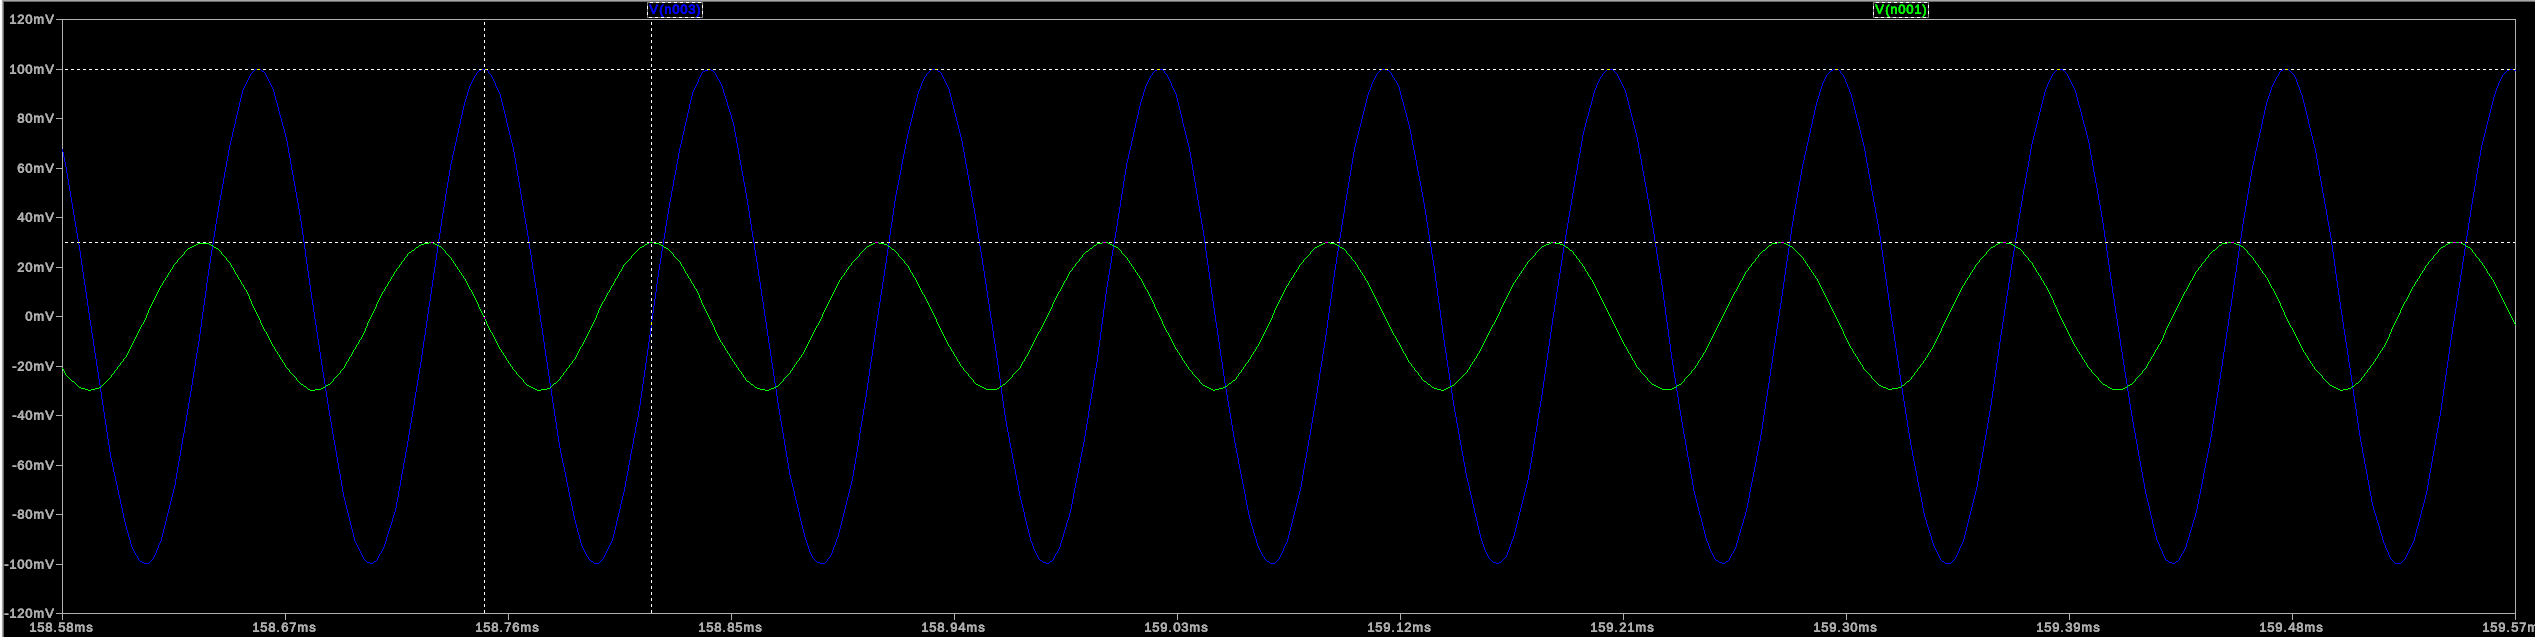
\includegraphics{ltfreq11000.png}
\end{adjustbox}

\begin{equation*}
    \begin{aligned}
         & V_f =          & 59.198177mV \\
         & V_i =          & 199.57788mV \\
         & Magnitude(H) = & 0.296616925 \\
         & Fase =         & -4.65829159
    \end{aligned}
\end{equation*}

\subsubsection{Tabela de resultados}



\subparagraph*{}

\begin{center}
    \begin{tabular}{ |c|c|c| }
        \hline
        Freq (Hz) & | H (jw) |  & Fase (H)      \\
        40        & 0.586186547 & $-1.68605608$ \\
        100       & 1.52323946  & $-1.60226153$ \\
        200       & 3.53268737  & $-1.67119113$ \\
        400       & 18.6104333  & $-2.06820459$ \\
        480       & 48.7670824  & $-3.1349102$  \\
        550       & 20.8160035  & $-2.01155708$ \\
        1100      & 3.6320926   & $-1.65494612$ \\
        2200      & 1.55687244  & $-4.68032157$ \\
        5500      & 0.595261852 & $1.60939706$  \\
        11000     & 0.296616925 & $-4.65829159$ \\
        \hline
    \end{tabular}
\end{center}
\newpage
\section{Medicoes em laboratorio}

\paragraph{Vamos inicialmente fazer as medicoes dos componentes a serem usados.}

\subsection{Tabela de componentes}

\begin{equation*}
    \begin{aligned}
        C_1 & = 104.89nF    \\
        C_2 & = 101.28nF    \\
        R_1 & = 465.1 omega \\
        R_2 & = 473.7 omega \\
        R_3 & = 46.25 omega \\
    \end{aligned}
\end{equation*}

\subsection{Medicoes no osciloscopio}

\subsubsection*{Analise em $40Hz$}
\subparagraph*{}

\begin{adjustbox}{scale=0.18}
    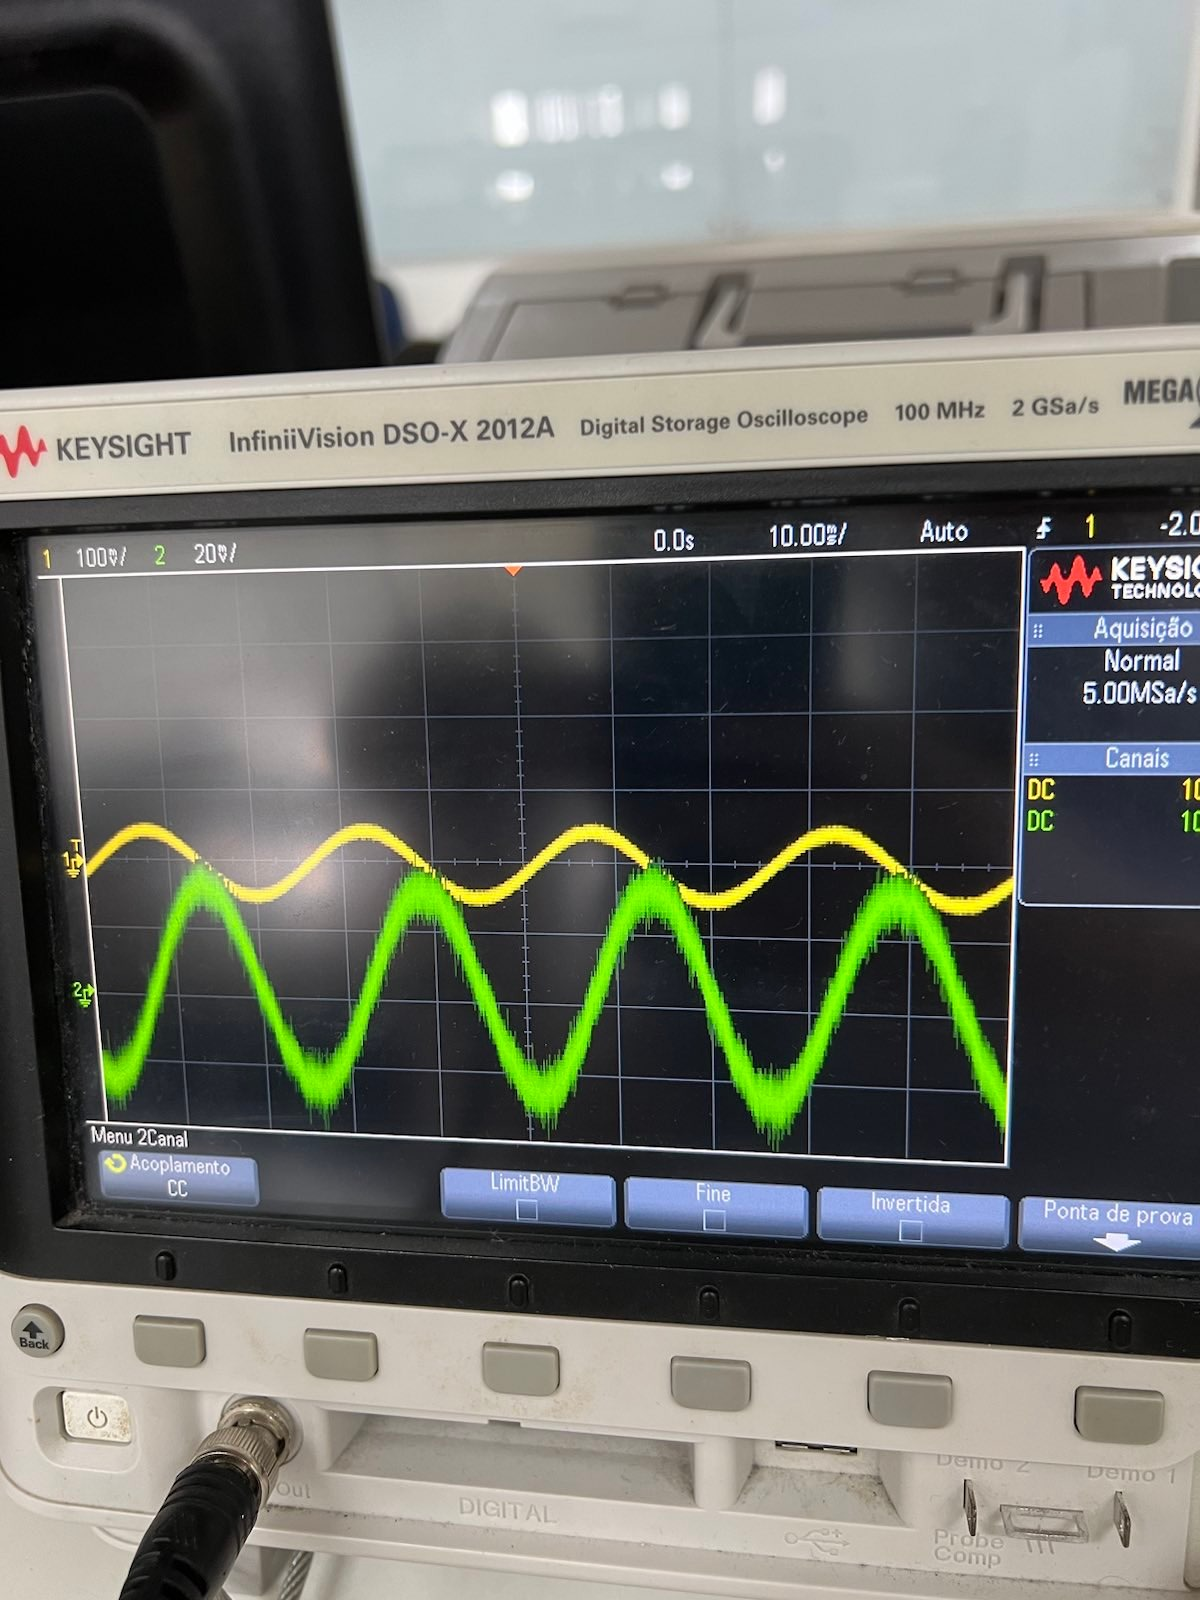
\includegraphics{freq40.jpeg}
\end{adjustbox}

\begin{equation*}
    \begin{aligned}
         & V_f =          & 0.565V     \\
         & V_i =          & 0.092V     \\
         & Magnitude(H) = & 0.473      \\
         & Fase =         & -1.5833627
    \end{aligned}
\end{equation*}


\subsubsection{Analise em $100Hz$}
\subparagraph*{}

\begin{adjustbox}{scale=0.18}
    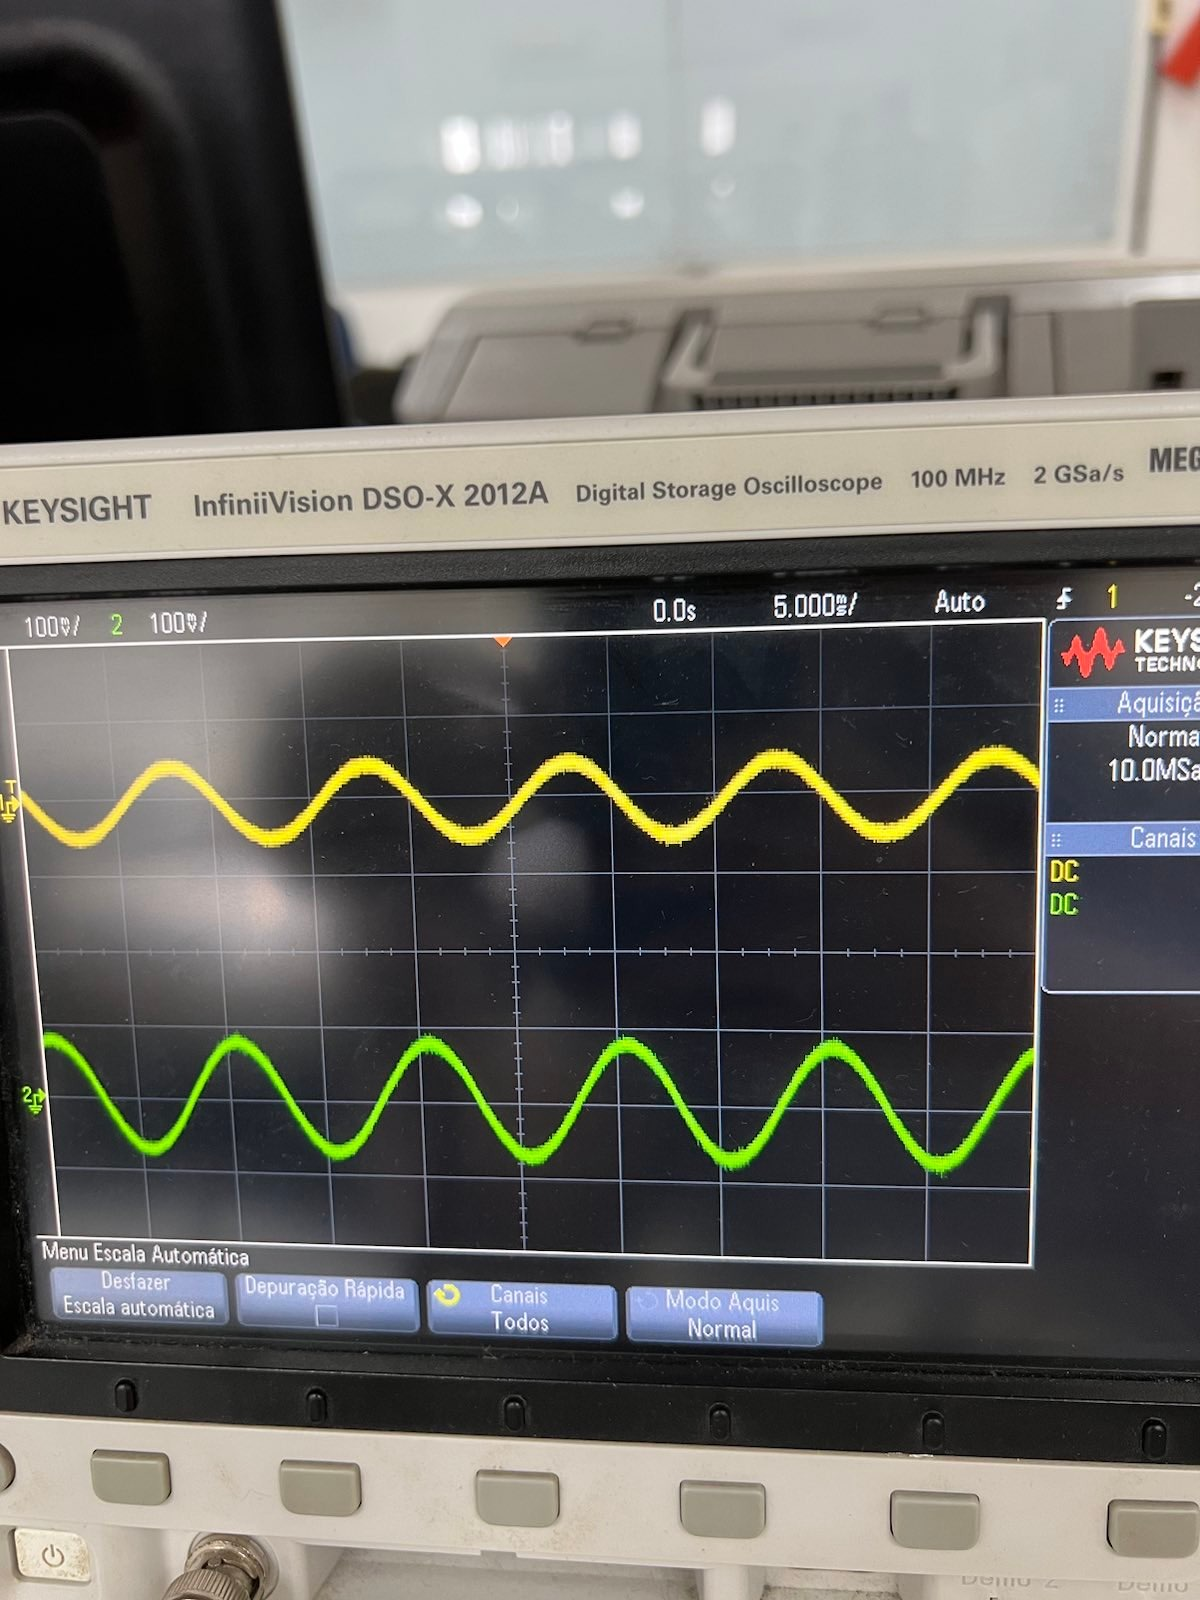
\includegraphics{freq100.jpeg}
\end{adjustbox}

\begin{equation*}
    \begin{aligned}
         & V_f =          & 1.52V       \\
         & V_i =          & 0.09425V    \\
         & Magnitude(H) = & 1.42575     \\
         & Fase =         & -1.57079633
    \end{aligned}
\end{equation*}

\subsubsection{Analise em $200Hz$}
\subparagraph*{}

\begin{adjustbox}{scale=0.18}
    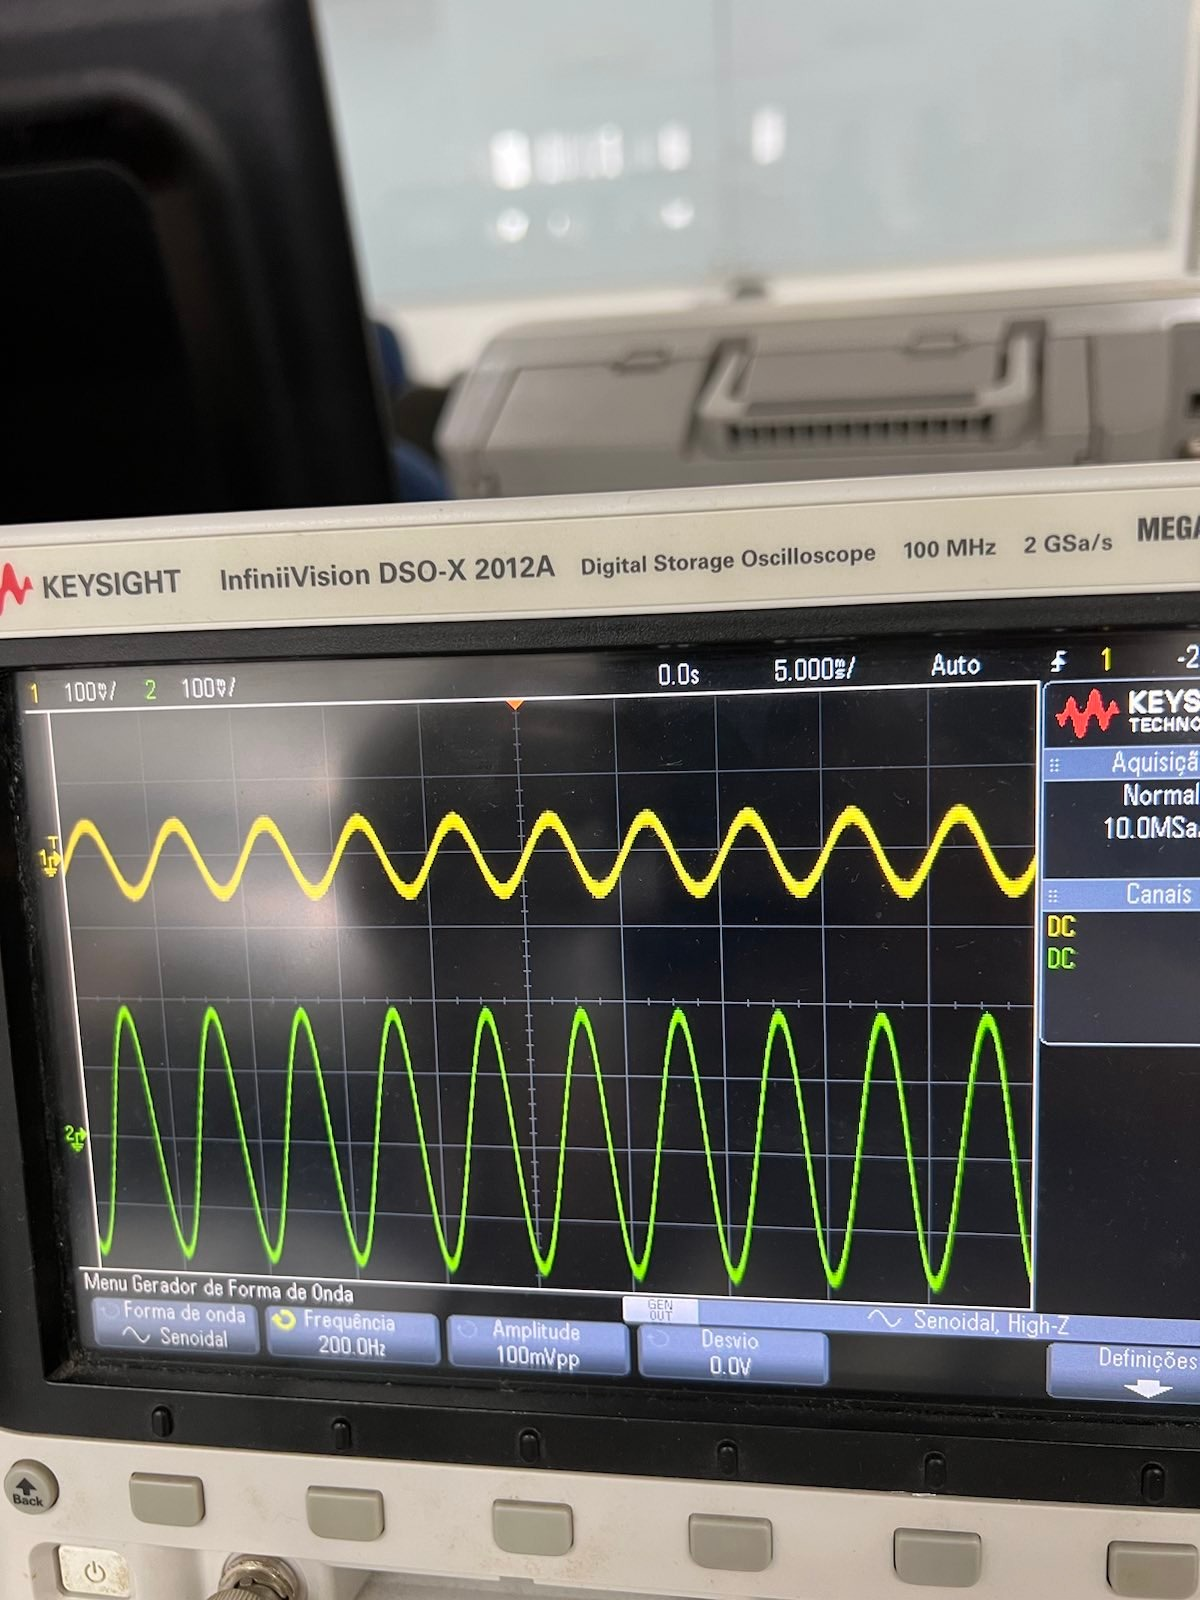
\includegraphics{freq200.jpeg}
\end{adjustbox}

\begin{equation*}
    \begin{aligned}
         & V_f =          & 3.5425V     \\
         & V_i =          & 0.097V      \\
         & Magnitude(H) = & 3.4455      \\
         & Fase =         & -1.55822996
    \end{aligned}
\end{equation*}

\subsubsection{Analise em $400Hz$}
\subparagraph*{}

\begin{adjustbox}{scale=0.18}
    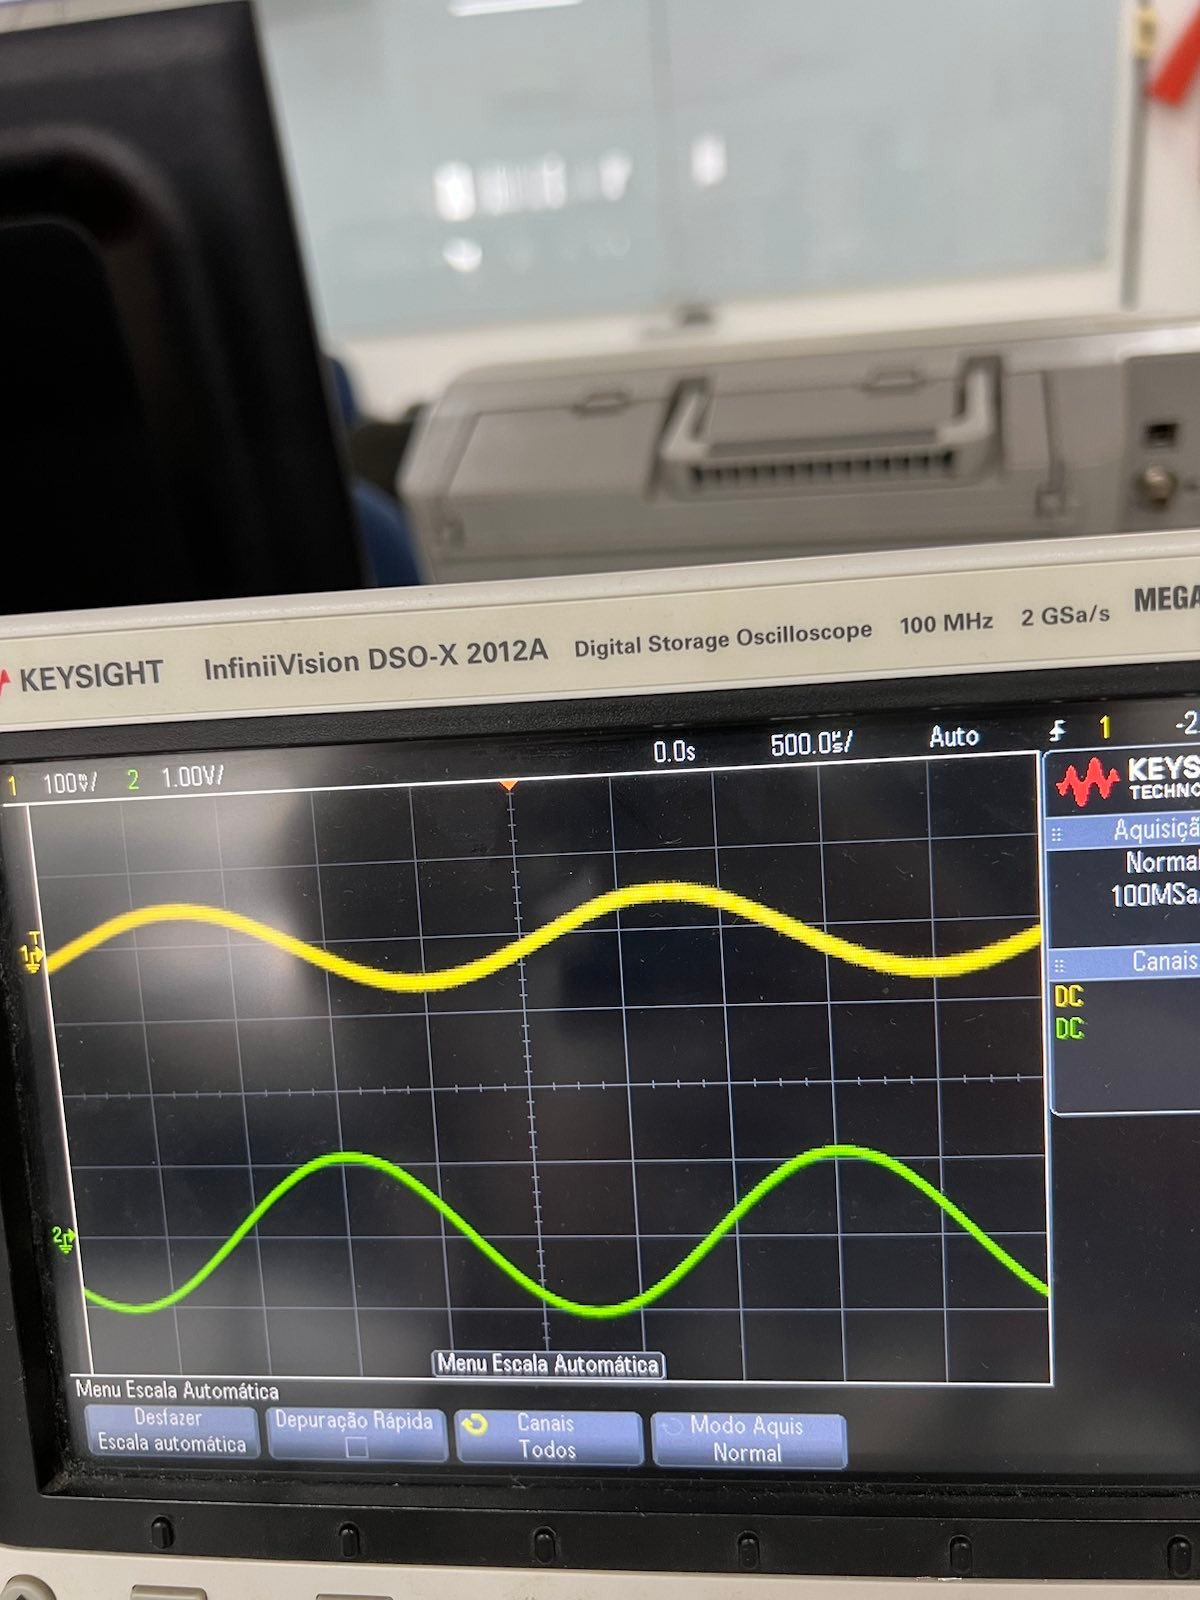
\includegraphics{freq400.jpeg}
\end{adjustbox}

\begin{equation*}
    \begin{aligned}
         & V_f =          & 21.5V       \\
         & V_i =          & 0.106V      \\
         & Magnitude(H) = & 21.394      \\
         & Fase =         & -1.98548656
    \end{aligned}
\end{equation*}

\subsubsection{Analise em $480Hz$}
\subparagraph*{}

\begin{adjustbox}{scale=0.18}
    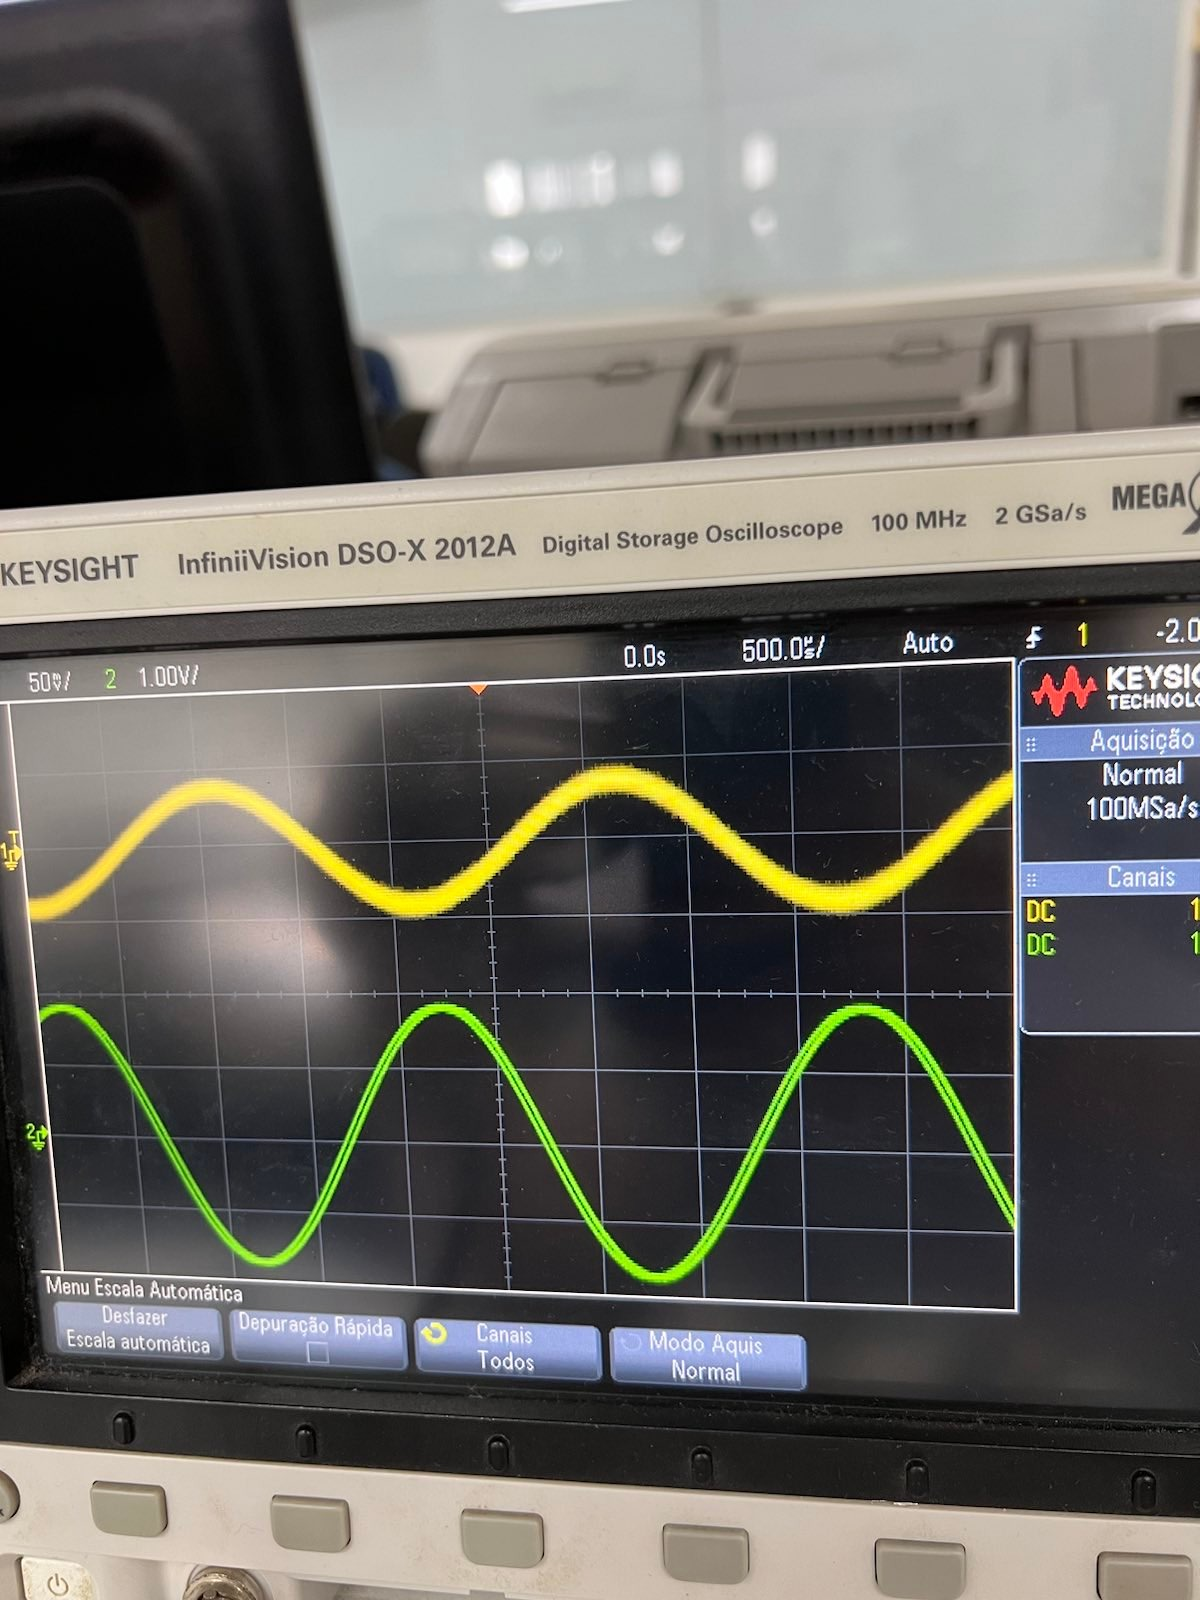
\includegraphics{freq480.jpeg}
\end{adjustbox}

\begin{equation*}
    \begin{aligned}
         & V_f =          & 36.75V      \\
         & V_i =          & 0.1V        \\
         & Magnitude(H) = & 36.65       \\
         & Fase =         & -3.40799971
    \end{aligned}
\end{equation*}

\subsubsection{Analise em $550Hz$}
\subparagraph*{}

\begin{adjustbox}{scale=0.18}
    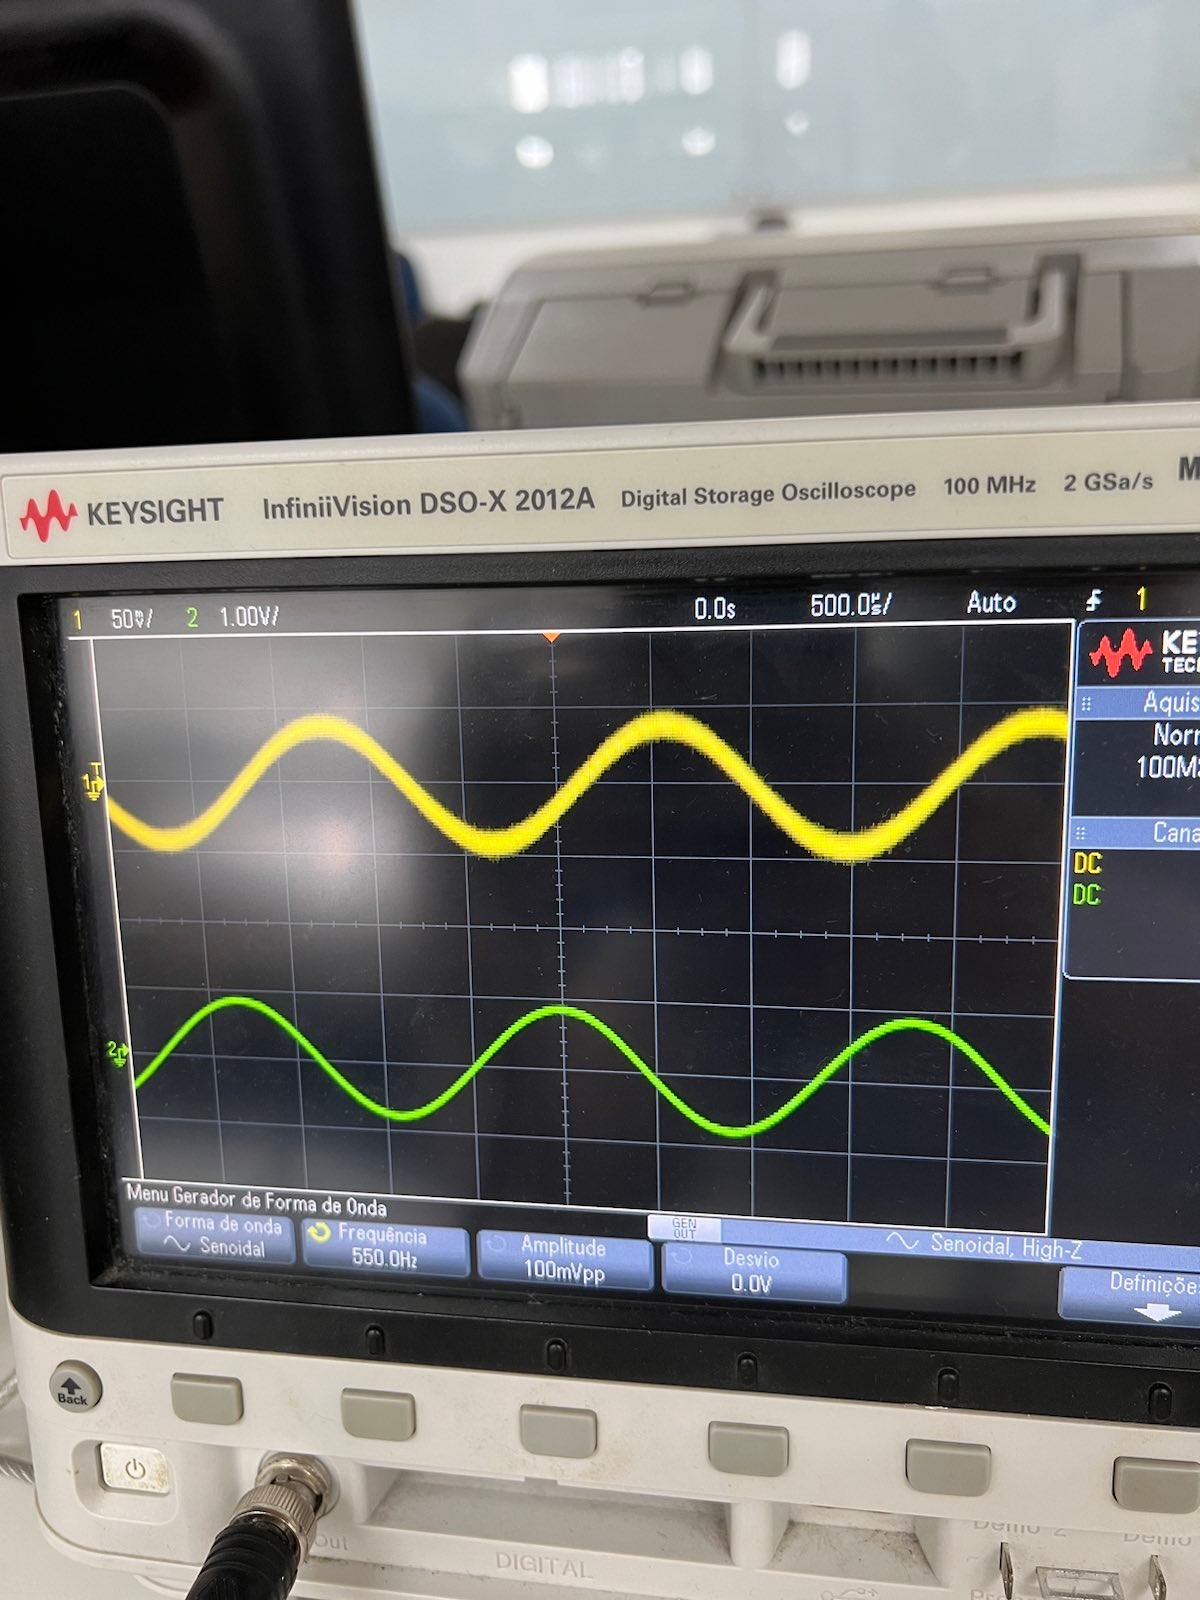
\includegraphics{freq550.jpeg}
\end{adjustbox}

\begin{equation*}
    \begin{aligned}
         & V_f =          & 16.8V      \\
         & V_i =          & 0.082V     \\
         & Magnitude(H) = & 16.71800   \\
         & Fase =         & 2.07345115
    \end{aligned}
\end{equation*}

\subsubsection{Analise em $1100Hz$}
\subparagraph*{}

\begin{adjustbox}{scale=0.18}
    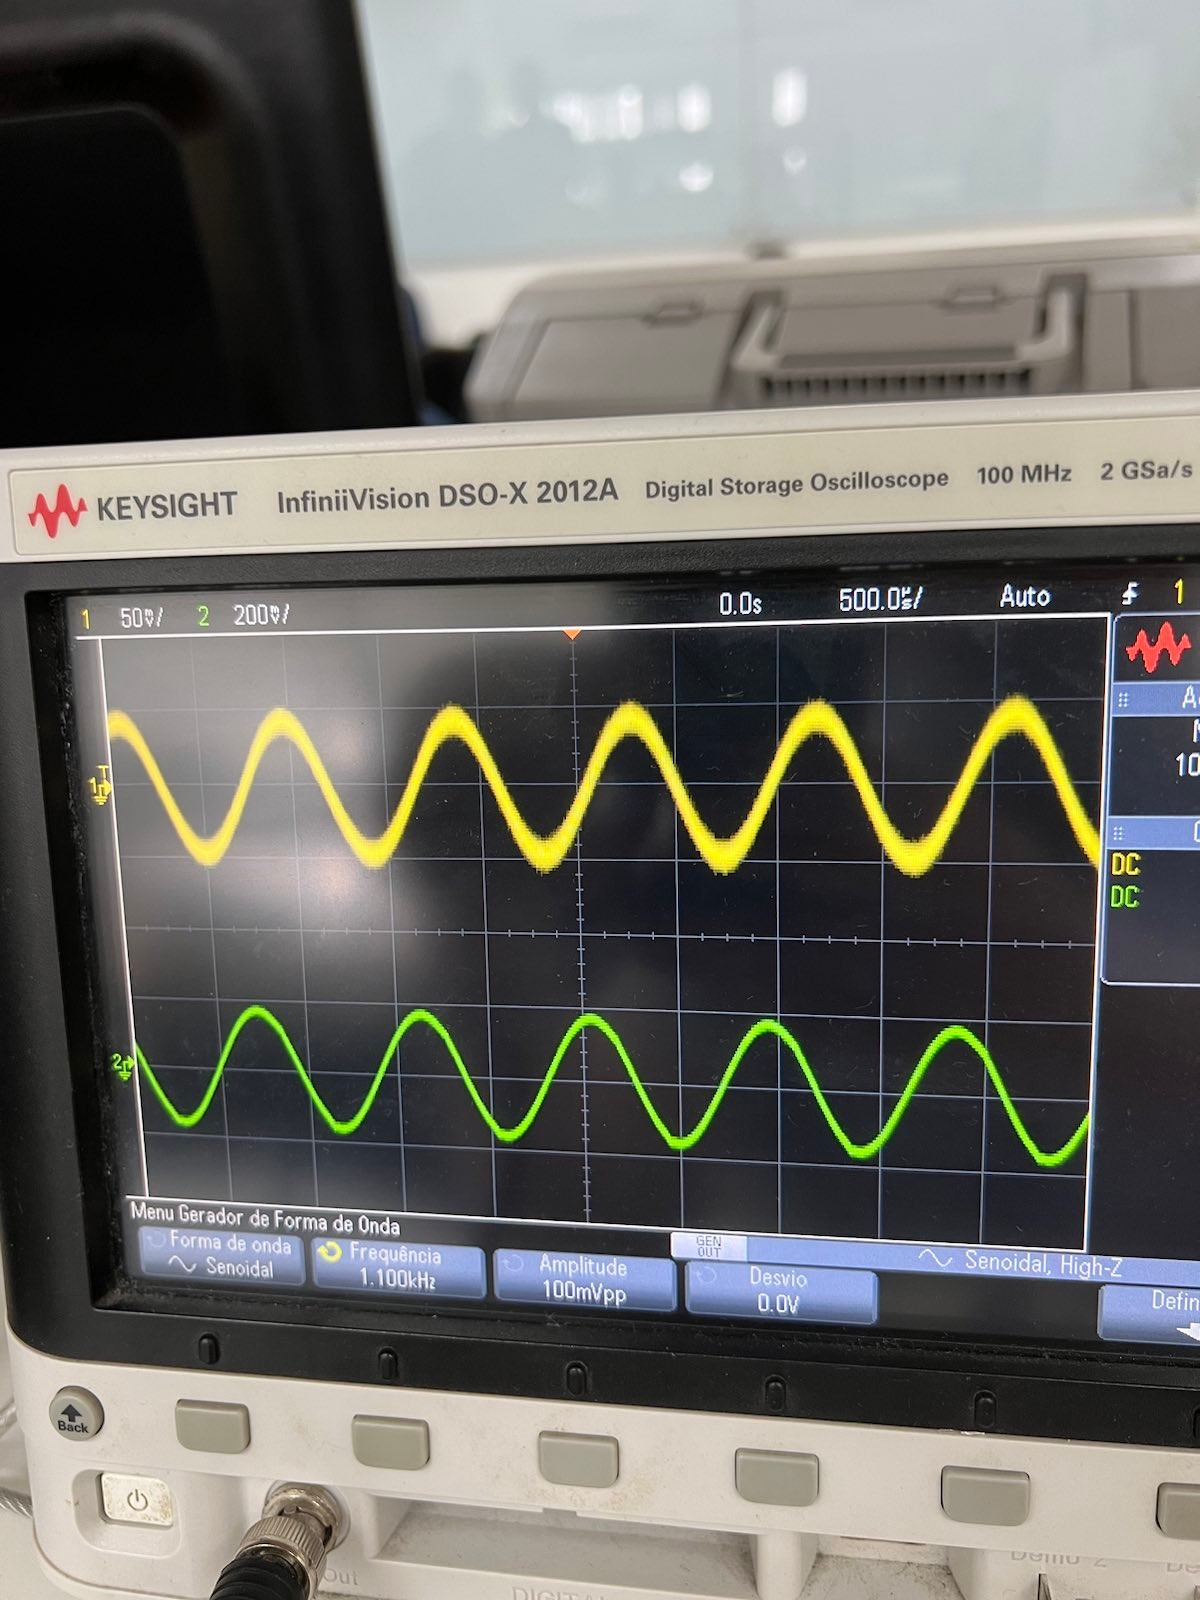
\includegraphics{freq1100.jpeg}
\end{adjustbox}

\begin{equation*}
    \begin{aligned}
         & V_f =          & 3.3175V    \\
         & V_i =          & 0.088V     \\
         & Magnitude(H) = & 3.2295     \\
         & Fase =         & 1.58964588
    \end{aligned}
\end{equation*}



\subsubsection{Analise em $2200Hz$}
\subparagraph*{}

\paragraph*{Eu achei que tinha tirado fotos das frequencias $2200Hz$ e $11000Hz$ mas nao consegui acha-las na confecção do relatorio.}

\begin{equation*}
    \begin{aligned}
         & V_f =          & 1.4675V    \\
         & V_i =          & 0.8925V    \\
         & Magnitude(H) = & 0.575      \\
         & Fase =         & 1.65876092
    \end{aligned}
\end{equation*}

\subsubsection{Analise em $5500Hz$}
\subparagraph*{}


\begin{equation*}
    \begin{aligned}
         & V_f =          & 0.7V        \\
         & V_i =          & 0.09V       \\
         & Magnitude(H) = & 0.61        \\
         & Fase =         & 0.552920307
    \end{aligned}
\end{equation*}


\subsubsection{Analise em $11000Hz$}
\subparagraph*{}


\begin{equation*}
    \begin{aligned}
         & V_f =          & 0.09V       \\
         & V_i =          & 199.57788mV \\
         & Magnitude(H) = & 0.04325V    \\
         & Fase =         & 1.24407069
    \end{aligned}
\end{equation*}

\subsubsection{Tabela de resultados}

\subparagraph*{}

\begin{center}
    \begin{tabular}{ |c|c|c| }
        \hline
        Freq (Hz) & | H (jw) | & Fase (H)      \\
        40        & 0.473      & $-1.5833627$  \\
        100       & 1.42575    & $-1.57079633$ \\
        200       & 3.4455     & $-1.55822996$ \\
        400       & 21.394     & $-1.98548656$ \\
        480       & 36.65      & $-3.40799971$ \\
        550       & 16.71800   & $2.07345115$  \\
        1100      & 3.6320926  & $ 1.58964588$ \\
        2200      & 0.575      & $1.65876092$  \\
        5500      & 0.61       & $0.552920307$ \\
        11000     & 0.04325    & $1.24407069$  \\
        \hline
    \end{tabular}
\end{center}

\subsection{Comparacao com valores teoricos}

\subparagraph*{Podemos ver que os valores de magnitude ficaram coerentes com ambas analises teoricas, e os de fases pra frequencias baixas tambem, mas tive problemas pra entender o sentido do sinal da fase a medida que a frequencia subia.}

\subsection{Graficos}

\subsubsection{Escala log-log da magnitude de H(jw) e f}

\begin{adjustbox}{scale=0.70}
    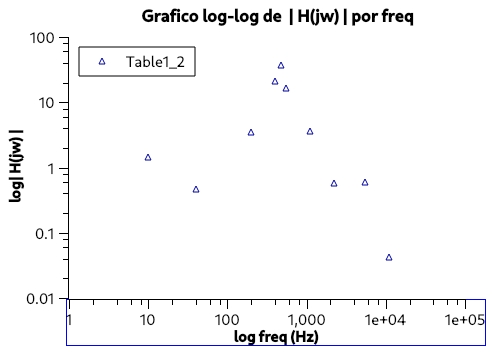
\includegraphics{Graph1.jpeg}
\end{adjustbox}

\subsubsection{Escala semilog da fase de H(jw) e f}
\begin{adjustbox}{scale=0.70}
    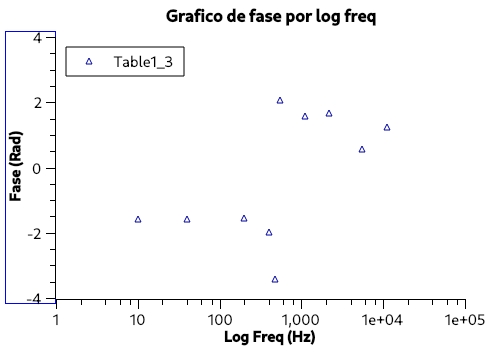
\includegraphics{Graph2.jpeg}
\end{adjustbox}

\section{Conclusões}

\subparagraph*{Conseguimos com sucesso fazer a analise numerica por dois meios, utilizando o LTSpice e WxMaxima, e comparamos os resultados.}

\subparagraph*{Nos resultados praticos, a magnitude da funcao transferencia foi coerente com os resultados esperados, porem a fase em frequencias baixas se manteve coerente, porem em frequencias altas ela se tornou inconsistente.}

\subparagraph*{Creio que por erros das minhas medidas, eu nao fui consistente em usar o mesmo cursor na mesma onda de entrada ou saida.}

\subparagraph*{A frequencia de saida comecou adiantada em relacao a frequencia de entrada, e a medida que aumentamos a frequencia ela se atrasa ate que eh ultrapassada pela entrada.}

\subparagraph*{Creio que isso faria com que a fase se inverta.}

\subparagraph*{Mas em suma creio que tivemos sucesso em nos familizariar com as ferramentas de analise de circuitos eletricos numericos.}

\end{document}